\chapter{O teste sistêmico na produção de placas de circuito impresso}
%todo falar de PCOLA/SOQ/FAM do iNEMI (International Electronics Manufacturing Initiative)

Os testes de circuitos eletrônicos fazem parte em toda a cadeia de projeto, fabricação e operação de um produto. Sua importância se nota desde as primeiras etapas de validação de um projeto de um sistema eletrônico, passando pelas etapas de produção de circuitos integrados, no controle de qualidade de um processo produtivo, e até mesmo no diagnóstico em campo do produto final. Como o presente trabalho discorre sobre testes de fim de linha, o foco será nas etapas de teste na cadeia produtiva.

\section{Teste e diagnóstico pela cadeia produtiva:do circuito integrado, ao teste sistêmico em campo}
 
O teste de circuitos inicia-se no teste de circuitos integrados, para verificar danos aos wafers de silício. Caracterizam-se pelo uso de jigas de teste complexas e uso de técnicas de projeto orientado à testabilidade (DfT), e também pela introdução de varredura perimétrica, autoteste embutido e compressão de dados de teste.

Por mais que os componentes integrados mais importantes de um sistema eletrônico já saiam de fábrica verificados, é também necessário validar as interações destes componentes com o restante da placa. Para isto temos as etapas de teste de placas de circuito impresso, que, felizmente possuem uma boa variedade de abordagens possíveis para a realização de testes, medições e inspeções. Muitas vezes a própria infraestrutura e funcionalidades de teste dos componentes integrados podem ser reutilizados no teste de placa, como as estruturas lógicas de varredura perimétrica. Dentre as técnicas específicas desta etapa destacam-se a inserção de pontos de teste, inspeções óticas e de raio-x automatizadas, o uso de camas de prego nas jigas de teste, e o uso do IEEE 1149.1, o JTAG, que é hoje o padrão de teste mais utilizado em placas de circuitos eletrônicos após a montagem de componentes na placa.

Nas etapas finais de montagem do produto final é necessário testar a integração da placa eletrônica com o restante do sistema. Importa aqui assegurar o desempenho dinâmico e funcional do sistema, com testes em velocidade de operação nominal para detectar problemas de temporização e a integração com o outros subsistemas do produto. O método mais comum e difundido para detectar problemas nesta etapa é através de testes funcionais e da execução da aplicação final. Nesta etapa é essencial que se tenha um bom diagnóstico do problema para a identificação e reposição do módulo defeituoso.

Mesmo com o produto em operação, as preocupações com teste e diagnóstico não cessam. É de grande interesse do fabricante e do cliente final a detecção de defeitos pós-produção com o produto em campo, assim como o monitoramento da saúde do sistema. Esta etapa é especialmente desafiadora, pois o acesso às ferramentas e instrumentos específicos de teste e diagnóstico é limitado ou até mesmo impossível. Dessa maneira, o desenvolvimento e implementação de ferramentas de auto-teste (BIST), auto-diagnóstico (BISD), e monitoramento são importantes para garantir as qualidades do produto e de operação do sistema.

Fala-se em diagnóstico, pois, muitas vezes, mesmo com testes apontando falhas, a causa raiz do problema pode não ser devidamente identificada. Isso é especialmente problemático quando o sistema está em operação, isso porque uma falha não devidamente tratada provavelmente retornará para a manutenção, gerando mais custos, e impedindo o processo de identificação da falha de fabricação ou projeto que, por sua vez, influencia na qualidade do produto.Este tipo de situação recebe diversos nomes, como \textit{No Failure Found, No Trouble Found, No Defect Found}.

Há ainda os casos aonde nem mesmo o teste consegue detectar a falha. Trata-se de um problema de cobertura de teste, que pode ser mensurada por métricas de teste e se baseia em modelos de falta.

Modelos de falta são separados em classes de: defeito materiais; defeitos em pinos e malha de circuito; problemas funcionais; e problemas de desempenho. 

\textit{Defeitos em materiais}  podem ser mensurados por métricas padrão de processo de qualidade, e exemplificados por defeitos em placas, processo de montagem: solda ruim terminal levantado, componente defeituoso, desalinhamento, efeito lápide.

Os \textit{defeitos a nível de pino e malhas de circuito} são modelados por análise estrutural e já possuem uma base bem estabelecida. Entram nessa classe as falhas de circuitos abertos ou em curto, defeito de driver (\textit{buffer}, pino).

Há ainda os problemas \textit{funcionais}, como falhas de \textit{boot}, cuja métrica são estabelecidas e investigadas por pesquisadores em desenvolvimento de software e lógica descritiva.
Por final, temos os problemas de desempenho em linhas de comunicação: alta taxa de erro, \textit{crosstalk, jitter, delay,} etc.

Apesar da dificuldade de estimar uma boa cobertura de falhas, a industria tenta cobrir as falhas com testes em materiais e montagem utilizando a inspeção de pasta de solda (SPI) a inspeção ótica automática (AOI) e a inspeção radiográfica automática (AXI); para falhas em pinos e malhas, verificação periférica \citet{ieee11491yr2013}, e \textit{in-circuit test (ICT)}; e testes funcionais para falhas de desempenho e operação. Esta relação entre testes estruturais e funcionais é descrita em \citet{thomaswenzelenricozimmermann2016} e sintetizada na figura \ref{fig:cobertura}. 

Todavia, essa segmentação vem mudando com os avanços nas técnicas de verificação periférica e de teste centralizado por microcontrolador, que incorporam boa parte dos testes de desempenho e até mesmo funcionais. Tais técnicas serão descritas nas sessão \ref{FCT}.

\begin{figure}[ht]
    \centering
    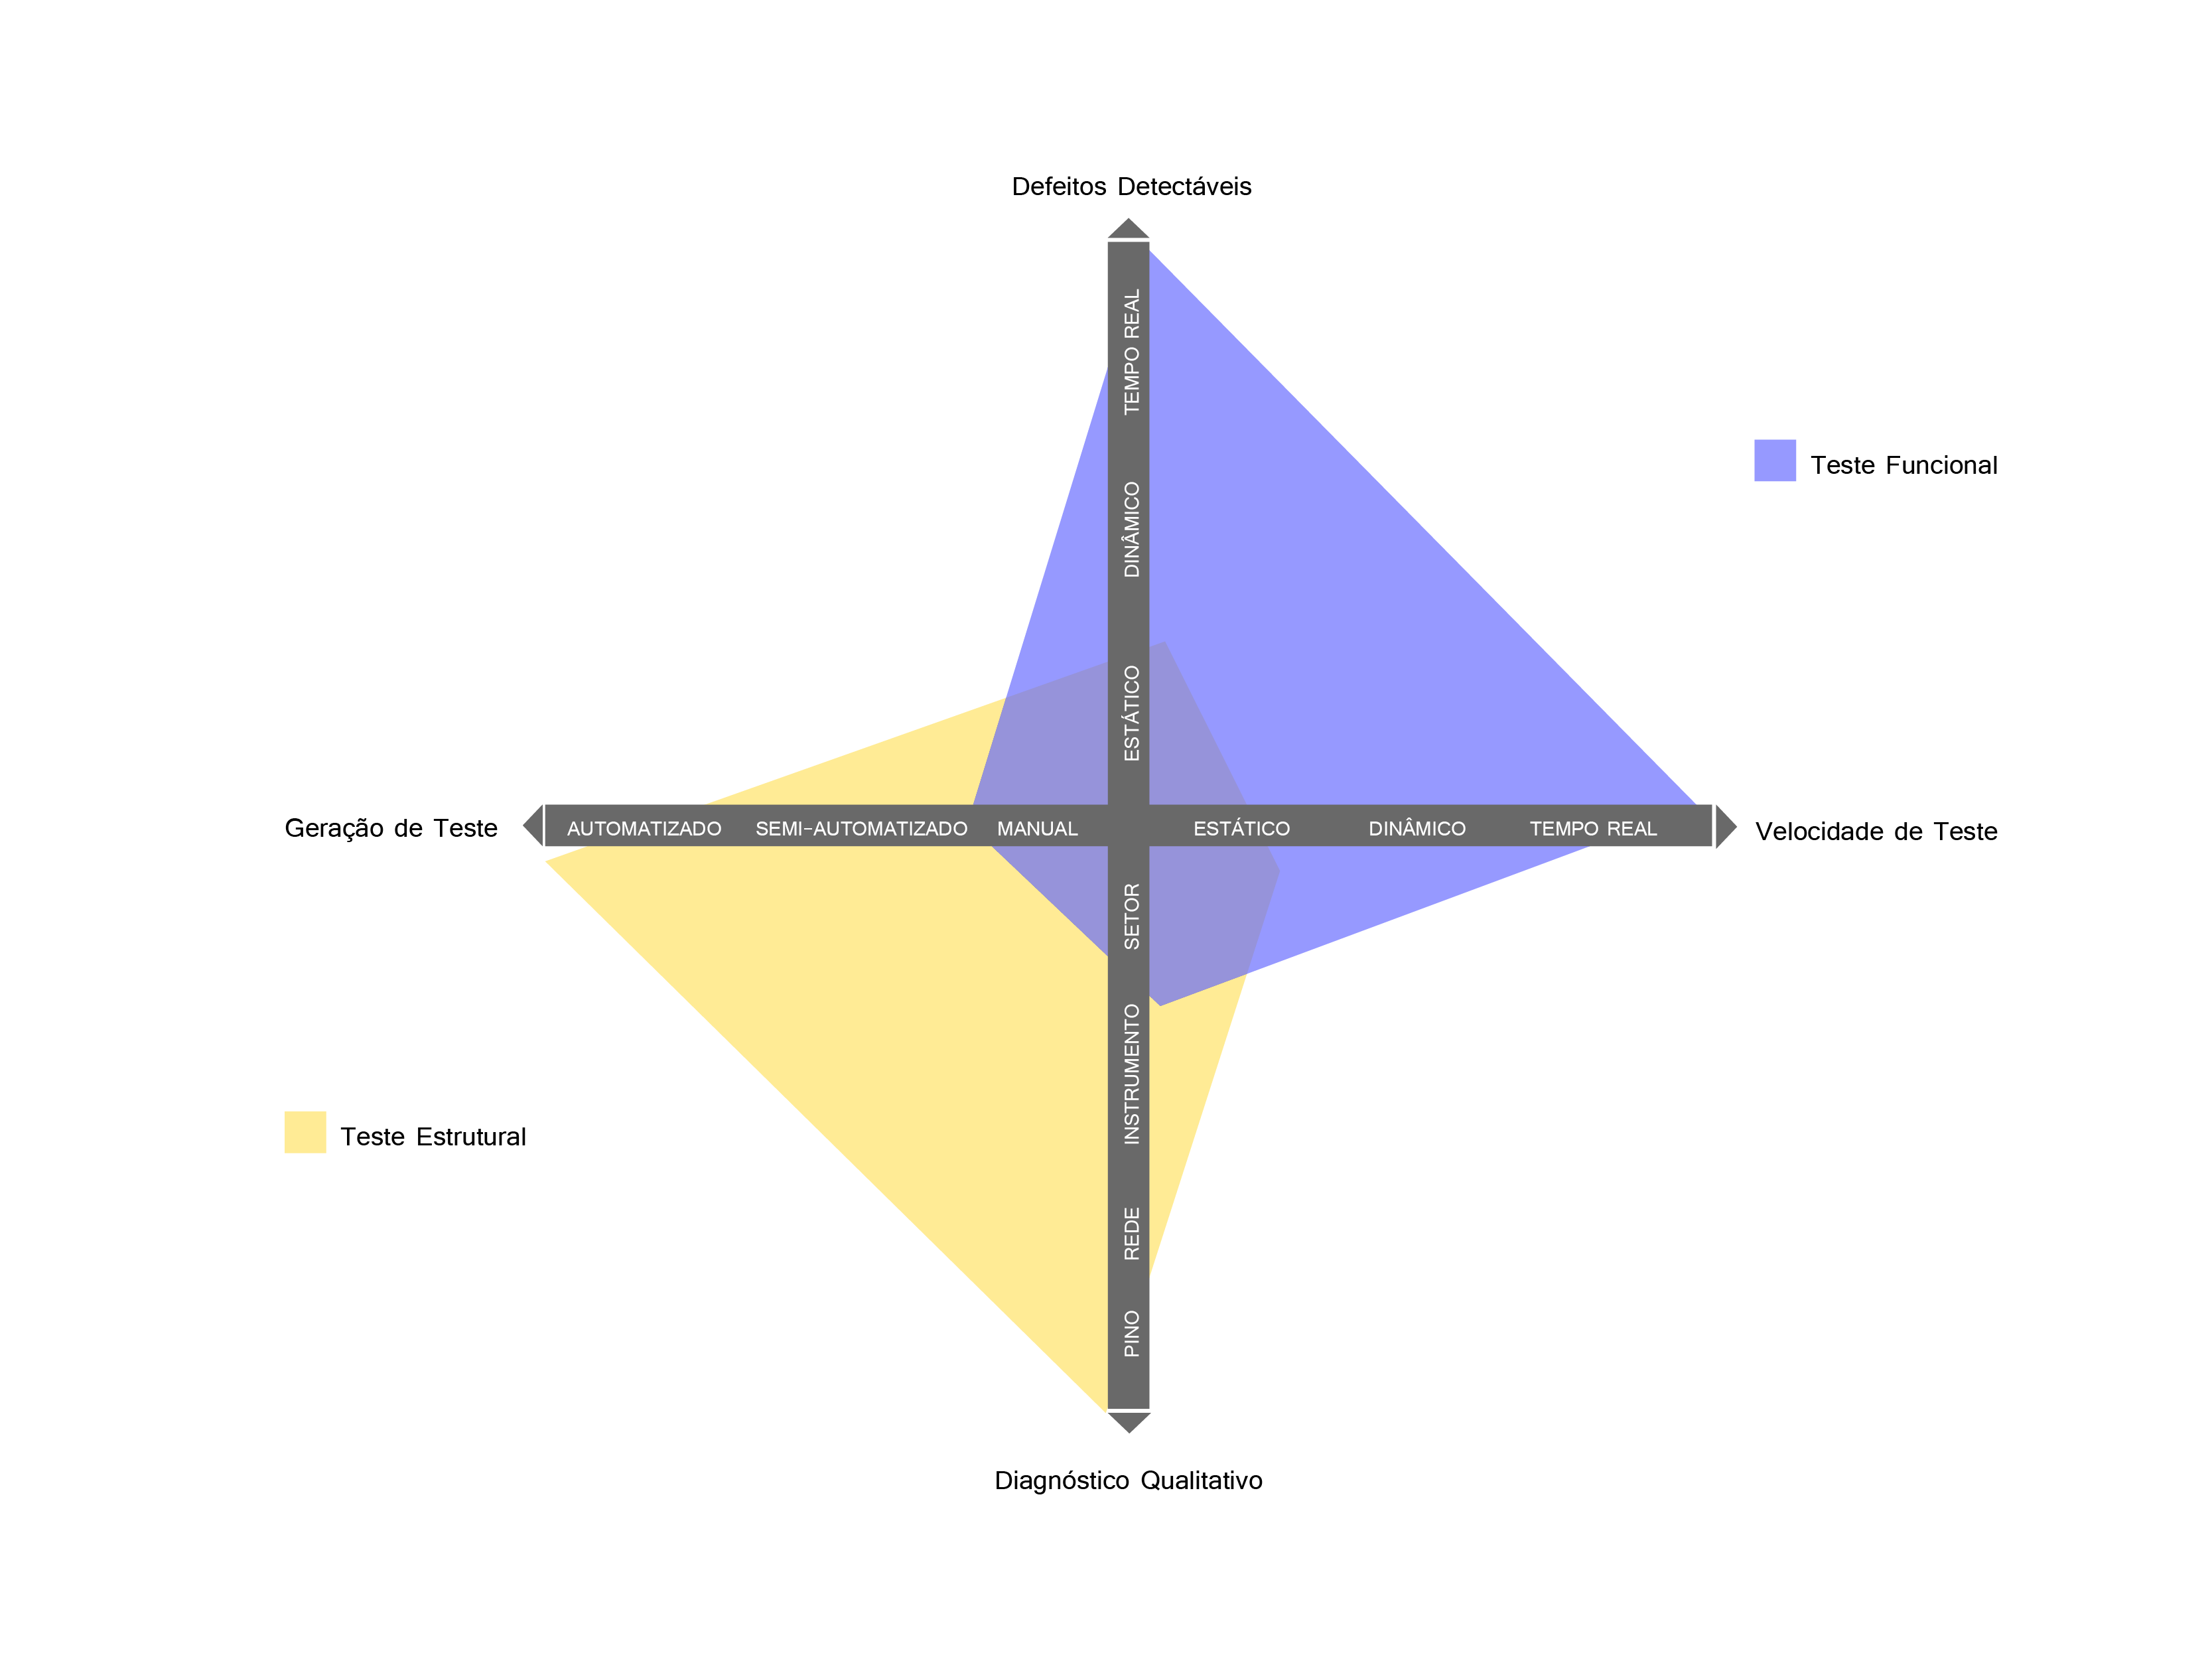
\includegraphics[width=1.1\linewidth]{coberturateste.png}
    \caption{A complementariedade dos testes estruturais e funcionais para a cobertura de teste de um dispositivo. Adaptado de \cite{thomaswenzelenricozimmermann2016}.}
    \label{fig:cobertura}
\end{figure}

Vimos aqui, portanto, que diversas técnicas e abordagens de teste e diagnóstico integram-se e são parte importante da produção, operação e manutenção de um sistema eletrônico. A seguir estas técnicas serão descritas detalhadamente. 

Ressalta-se que a cadeia de testes é facilitada pela reutilização das ferramentas e infraestrutura de testes utilizadas pelas etapas anteriores. Um bom exemplo disso são os autotestes utilizados na validação pós-silicone dos SoCs que podem ser reutilizados tanto na validação de placas em linha de produção, como em campo no diagnóstico de problemas de placa.

\subsection{Inspeção de Pasta de Solda}

A inspeção de pasta de solda é o processo, normalmente automático, de achar falhas após a aplicação da pasta de solda. A inspeção de pasta de solda previne o retrabalho de placas com os componentes montados, por que, uma vez com os erros de solda detectados, a placa defeituosa pode ser separada das demais. A detecção de falhas ainda nesta etapa custa 10 vezes menos do que uma falha pós refusão, ou após a solda, e 70 vezes menos que uma falha no teste elétrico \textit{In-circuit} \citep{owen2000process};

Os sistemas mais simples de inspeção de pasta de solda consistem de uma imagem colorida da placa. Este método consegue detectar ausência de solda e conexões indevidas entre blocos vizinhos, porém, por ser um método 2D, não consegue estimar a altura e volume da pasta de solda. Isso pode gerar problemas indetectáveis em outras etapas, já que, por mais que passe em testes de condutividade, a falta de pasta de solda em uma conexão pode causar problemas mecânicos e rompimento da interconexão. 

O volume de pasta de solda pode ser estimado por diversos métodos. \citet{5246351} introduz as principais tecnologias de perfilometria: 
\begin{itemize}
    \item Triangulação a laser;
    \item Perfilometria por fase, utilizando luz estruturada;
    \item Reconstrução por Redes Neurais;
\end{itemize}

Os métodos por triangulação a laser utilizam-se das projeções do feixe laser no relevo da placa para reconstruir o seu perfil 3D.  \cite{5576321} descreve os detalhes desta técnica. Medições precisas podem ser obtidas com este método, entretanto são equipamentos caros, com baixa velocidade de inspeção, e susceptíveis a ruídos refletivos e \textit{efeito de sombras} \citep{5246351}.

Na perfilometria por fase, uma luz estruturada projeta um padrão, como uma grade ou uma série riscos, na PCI com a pasta de solda aplicada. Este padrão é então pouco a pouco deslocado e uma série de imagens são capturadas por uma câmera de alta resolução. Os sistemas mais avançados empregam um sistema livre de sombras onde ambos os lados da deposição de solda são caracterizados simultaneamente. \cite{5576321} oferece uma abordagem para o problema das sombras, e \cite{5246351} faz uma revisão dos principais trabalhos em perfilometria por fase.

O método de reconstrução por redes neurais tenta resolver os problemas do \textit{shape-from-shading (SFS)}, que até então era um método cujo desempenho era inconsistente. \cite{5246351} revisa o estado da arte e propõe uma nova abordagem.

% http://www.circuitnet.com/news/uploads/1/Vi_Technology_3D_SPI_Article.pdf

\subsection{inspeção ótica automática - AOI}
% inserir https://repositorio.ufsc.br/xmlui/bitstream/handle/123456789/158843/337436.pdf?sequence=1&isAllowed=y

A inspeção ótica automática (AOI), como o próprio nome indica, inspeciona visualmente a placa de circuito por meio de fotos, processa e identifica automaticamente as falhas, seja de componente ou solda. Esta técnica é usada para detectar componentes trocados, faltantes, ou mal posicionados, e pode ser realizada na etapa pré-forno de refusão ou após, dependendo da particularidade do processo produtivo da fábrica. O trabalho de \cite{huang2015automated}, citado por \cite{mello2015sistema} indica quatro categorias de inspeção ótica automática:

\begin{itemize}
    \item \textbf{Métodos de projeção}, que correlacionam a entrada com modelos aprendidos e suas características;
    \item \textbf{Abordagem baseada em filtro:} filtro espaciais com base em transformadas de sinal, como por exemplo Fourier, Wavelet, discreta cosseno;
    \item \textbf{Aprendizagem de máquinas:} Os mais utilizados são as redes neurais, algoritmos genéticos, e máquinas de vetor suporte;
    \item \textbf{Abordagens híbridas:} associam diversas técnicas para classificações mais complexas. 
\end{itemize}

%A AOI na etapa pré-forno detecta componentes faltantes ou componentes errados, e alinhamento correto de componentes. Como este processo é realizado após a refusão, os defeitos são relativamente simples de corrigir e menos custosos do que após a etapa de refusão. Outra vantagem é que os problemas de calibração na máquina de posicionamento de componentes podem ser mais facilmente detectados e analisados. Uma análise de tendência nas etapas pós refusão não seria tão confiável, pois o processo de refusão altera a localização dos componentes, e problemas de calibração na máquina de posicionamento só seriam detectados após um aumento significativo de placas defeituosas.

%Na etapa pós refusão, a inspeção ótica automática é provavelmente a etapa mais aceita entre os fabricantes de placas eletrônicas. Um sistema AOI colocado nesta etapa detecta qualquer problema gerado ao longo do processo, incluindo defeitos de colocação de componentes e problemas relacionados à solda, como: falta ou excesso de solda, curto-circuitos ou circuitos abertos. Nesta etapa, a AOI detecta defeitos causados por problemas de impressão, pelo sistema de colocação de componentes, e ainda, pelo processo de refusão. O propósito da AOI após o processo de refusão não é somente prover dados de defeito necessários para o retrabalho de uma PCI, mas também para a coleta de dados através de múltiplas montagens de placa para análise de causa raíz e melhoramento contínuo da produção.

A maior limitação da AOI é a impossibilidade de detecção de defeitos em pinos ou partes do circuito não visíveis, como abaixo de componentes \textit{Ball Grid Array} (BGA) ou em circuitos eletromagneticamente blindados, nesses casos, é necessário o uso de outras ferramentas como a verificação de placas por radiografia.
\cite{savage1993automated} citado por \citep{mello2015sistema}
%todo
\subsection{Inspeção radiográfica automática - AXI}

A inspeção radiográfica automática (AXI), possui uma vantagem única em relação às outras tecnologias de inspeção estrutural: os materiais absorvem os raios-x proporcionalmente à sua massa atômica. A solda utilizada na montagem das PCIs consistem de materiais pesados como o chumbo e a prata. A maioria restante dos materiais usados na fabricação das PCIs são compostos por elementos leves como carbono, silício, alumínio, oxigênio, hidrogênio e cobre. Dessa forma, a inspeção radiográfica mostra-se muito interessante na geração de imagens do processo de solda: os pontos de solda aparecem muito bem, enquanto o restante da placa apresenta-se transparente. Outra vantagem é a possibilidade de inspecionar os pinos escondidos de encapsulamentos complexos como o BGA ou o \textit{chip-scale packages} (CSP), além de exibir características internas dos pontos de solda.

Segundo o trabalho de \citet{leinbach2001and}, apesar de sua superioridade, a inspeção radiográfica automática ainda não tem muita adesão devido ao seu preço, já que fontes de raio-x e detectores não são tão disponíveis quanto câmeras e fontes de luz, além dos requisitos computacionais necessários para processar as imagens. Ademais, a inspeção ótica automática ainda é mais rápida do que a radiográfica.

\subsubsection{Casos onde a inspeção radiografia é importante}

\citet{leinbach2001and} resume três casos aonde a inspeção radiográfica se faz importante.

Primeiro, na inspeção de componentes ocultos. Por utilizarem encapsulamentos CSP e BGA ou blindagem RF, um número crescente de placas caem dentro desta categoria. São exemplos os celulares, e outros produtos que utilizam comunicação sem-fio, onde muitos componentes são colocados dentro de uma área blindada e somente acessíveis por inspeção radiográfica.

Segundo, em placas com grande número de interconexões. Por mais refinado que seja o processo de fabricação, muitos  podem ocorrer. Sistemas de \textit{in-cirtuit test}, além de custosos para placas complexas, possuem uma taxa de falha de detecção que nestes casos seriam muito significativas. A inspeção radiográfica associada a um sistema de ICT podem melhorar a cobertura de testes e garantir o rigor do processo.

Terceiro, Em placas que precisam trabalhar em ambientes hostis ou em aplicações que requerem alta confiabilidade, a inspeção radiográfica garante um ótimo perfil da qualidade de solda. Isso é importante quando a placa precisa operar em ambientes com estresses mecânicos e térmicos que possam comprometer soldas mais fracas. Um bom exemplo seria um sistema embarcado automobilístico, onde uma solda fraca, dificilmente detectável em outros testes, pode-se romper em campo pela próprias vibrações do veículo em operação e o sistema falhar, causando um acidente.

Ainda que boa na inspeção de solda, no processo de montagem, a AXI desempenha melhor depois que todas as etapas de solda por onda tenham ocorrido. Pareada com técnicas de ICT a maior parte dos defeitos podem ser cobertos. O trabalho de \citet{oresjo2002use} comenta melhor a relação entre AOI, AXI, e os \textit{in-circuit testers - ICT}.

\subsubsection{Tipos de AXI}

 Há três tipos principais de AXI utilizados na manufatura \citep{dougmcclure2000}: a inspeção 2D, a tomosíntese digital e a laminografia 3D. 

A técnica mais usada é a inspeção 2D, que é semelhante à radiografia convencional porém, ao invés de uma chapa de raio-x como resultado final, as imagens digitalizadas e analisadas automaticamente. É melhor aplicada em placas com soldas em um só lado da placa. Em placas com junções de solda em alta densidade ou em ambos os lados a imagem gerada pode ficar confusa. 

Na tomosíntese digital, múltiplas radiografias tiradas em diferentes ângulos são processadas reconstruindo uma imagem 3D do objeto de estudo, possibilitando a análise de placas com soldas em ambos os lados e de alta densidade. A desvantagem desta técnica está na alta potência computacional requerida, que escala com o número de imagens usadas. Ao mesmo tempo o uso de poucas imagens pode causar erros e distorções que prejudicam o diagnóstico. Os avanços computacionais tem ajudado a tomosíntese a ganhar mercado, mas, ainda assim, é uma tecnologia que tem dificuldade em se manter competitiva em relação às outras, por sua baixa velocidade de teste.

Por último, temos a laminografia 3D, onde o emissor e o detector rotacionam sincronizadamente em volta da placa, defasados em 180 graus. A diferença entre esta técnica e a tomosíntese, é que na laminografia é mais fácil isolar um recorte da placa no eixo Z, tornando-a consideravelmente mais produtiva do que a tomosíntese.

\subsection{\textit{In-Circuit Testers (ICT)}}

Jigas de teste são uma grande ferramenta de teste de placas de circuito eletrônicas. Por meio de pontas de teste, pode-se obter acesso a pontos internos do circuito como também testar componentes isoladamente, separando-os de outros circuitos. Por meio de ICT, é possível detectar componentes defeituosos ou faltantes, circuitos abertos ou em curto, e até mesmo componentes errados. O ICT trabalha testando partes isoladas da placa, medindo resistência, capacitância, e em alguns casos indutância de subcircuitos da placa, normalmente acessíveis por conectores, pads, ou test points. Dessa forma, consegue-se realizar testes estruturais e até mesmo funcionais sobre o circuito podendo garantir que o mesmo foi fabricado corretamente e é funcional. Muitas vezes o ICT é usado também para a gravação de \textit{firmware} nas placas.OS ICT são compostos pelos seguintes elementos \citep{ianpoole2017}:

\begin{itemize}
    \item O ICT em si: composto por uma matriz de pares de acionadores e sensores que são usados para realizar as medições. Podem ser em torno de centenas, ou até milhares por ICT.
    \item A jiga de teste (\textit{fixture} ou fixação):  é a interface entre o ICT e a placa testada, roteando as entradas e saídas do ICT com o Dispositivo em Teste, através de pinos, num arranjo conhecido como cama de pregos.
    \item O software de teste: Software com a rotina de testes, e condições de aprovação/reprovação.
\end{itemize}

Dentre os três, somente o ICT em si não é customizado para cada placa. O sistema de jiga de testes por ser relativamente caro, é mais bem aplicado a grandes volumes de produção. Uma análise de custos deve de ser realizada para garantir que os custos de montagem da jiga e do programa são viáveis. 

\subsubsection{Tipos de ICT}

A tabela \ref{table:tiposdeict} sintetiza três categorias principais de testadores \citep{ianpoole2017}: O ICT tradicional; O \textit{flying probe test - FPT} cujas pontas de prova são controladas por comando numérico computadorizado (CNC); e o Analisador de Defeito de Fabricação: versão mais enxuta do ICT com funcionalidades reduzidas. 

\begin{table}[h!]
\centering
\caption{Tipos de ICT}
\label{table:tiposdeict}
{\footnotesize 
\begin{tabularx}{\textwidth}{@{} Y Y Y Y @{}}
\toprule
  \textbf{Tipo de ICT} & \textbf{Princípio de \mbox{Funcionamento}}  &\textbf{Vantagens}  &\textbf{Desvantagens} & \\ \midrule
\textbf{ICT tradicional} & - Pares de I/O em grande número; 

- Fixação e cama de pregos feitos sob medida. & - Alta velocidade de execução de teste; 

- Capacidade para medição de capacitância e indutância. & - Inviável para pequenas produções;

- Custo adicional para qualquer atualização da jiga;  \\ \addlinespace
\textit{\textbf{Flying probe test (FPT)}} & - Pontas de prova móveis e controladas por CNC; 

- A fixação de placa é genérica;
 & - Dispensa uma jiga de teste e cama de pregos; 
 
 - Alterações realizadas via software;
 & 
- Número limitado de pontos de testes simultâneos; 

- Baixa velocidade de teste; & \\ \addlinespace
\textbf{Analisador de Defeitos de Fabricação}
 & - Similiar ao ICT padrão, mas com funções limitadas.
 & - Alta velocidade de teste e custo reduzido;
 & - Limita-se a testes de continuidade e resistência elétrica.
  & \\ \bottomrule
\end{tabularx}}
\end{table}

\subsubsection{Cobertura de falta}
Em sua tese, \citet{de2008apoio} relata que os testes funcionais e estruturais realizados por ICT foram progressivamente dificultados por duas questões: 

A primeira é a miniaturização dos circuitos e componentes com valores muito baixos, cuja checagem de presença e valores é comprometida  devido à influencia de capacitâncias parasitas do próprio testador. O mesmo acontece com as indutâncias mas, ao menos, é possível detectar a presença do componente através da medição de resistência elétrica.

O segundo problema, e também o mais grave, é relacionado ao acesso aos nós do circuito. Seja pelas dimensões reduzidas da placa sob teste, que dificultam a construção de uma cama de pregos correspondente, como também pela completa inacessibilidade à uma região eletromagneticamente blindada ou à pinos inacessíveis de encapsulamentos de alta densidade, como os BGAs, que, hoje em dia, estão quase sempre presentes em placas de circuito impresso.

Estes fatores deram origem ao desenvolvimento da infra-estrutura normatizada de varredura periférica IEEE 1149.1 \citep{ieee11491old} para facilitar o teste de integrados digitais, e nas ultimas décadas se expandiu em outros padrões que cobrem desde medições analógicas a testes de canais de comunicação. 

\subsection{Varredura periférica}

Testes de varredura periférica (\textit{boundary scan}) como o \textit{Joint Test Action Group - JTAG} são hoje o padrão da indústria em teste de placas de circuito impresso e vem ao longo dos últimos anos substituindo os ICT. Isso se deve ao custo baixo desta tecnologia e eficiência em termos de cobertura de testes.
Os esforços para a criação do primeiro padrão de varredura periférica surgiu na década de 80 pelo grupo de mesmo nome, \textit{Joint Test Action Group - JTAG}, devido às crescentes dificuldades em criar ICTs para placas com componentes em alta densidade, dificuldade na inserção de pontos de teste no leiaute de circuito impresso, como também a distribuição de componentes em ambas as superfícies. Os esforços deste grupo de pesquisa resultou no padrão \citet{ieee11491old} em 1990, que obteve rápida adoção pela indústria eletrônica. Sua revisão mais atual é a \citet{ieee11491yr2013}.



Embora as primeiras aplicações do JTAG fossem direcionadas para teste de placas de circuito impresso, hoje o padrão também cumpre um papel essencial na depuração de sistemas embarcados graças ao acesso de baixo nível às entradas/saídas e estados internos do circuito integrado, fornecendo um meio barato e confiável de depuração.
A porta JTAG também serve para a gravação de \textit{firmware} na memória flash \citep{ieee1532}, sendo uma alternativa mais rápida ao uso de portas seriais e \textit{bootloaders}. 

Outra aplicação desta interface é a geração de testes automatizados para diagnóstico de placa em campo no conceito de BIST, ou auto teste embutido, possibilitando que uma placa faça auto-diagnóstico de problemas, como em circuitos periféricos. Estes conceitos serão abordados no próxima seção deste trabalho.

\begin{figure}
    \centering
        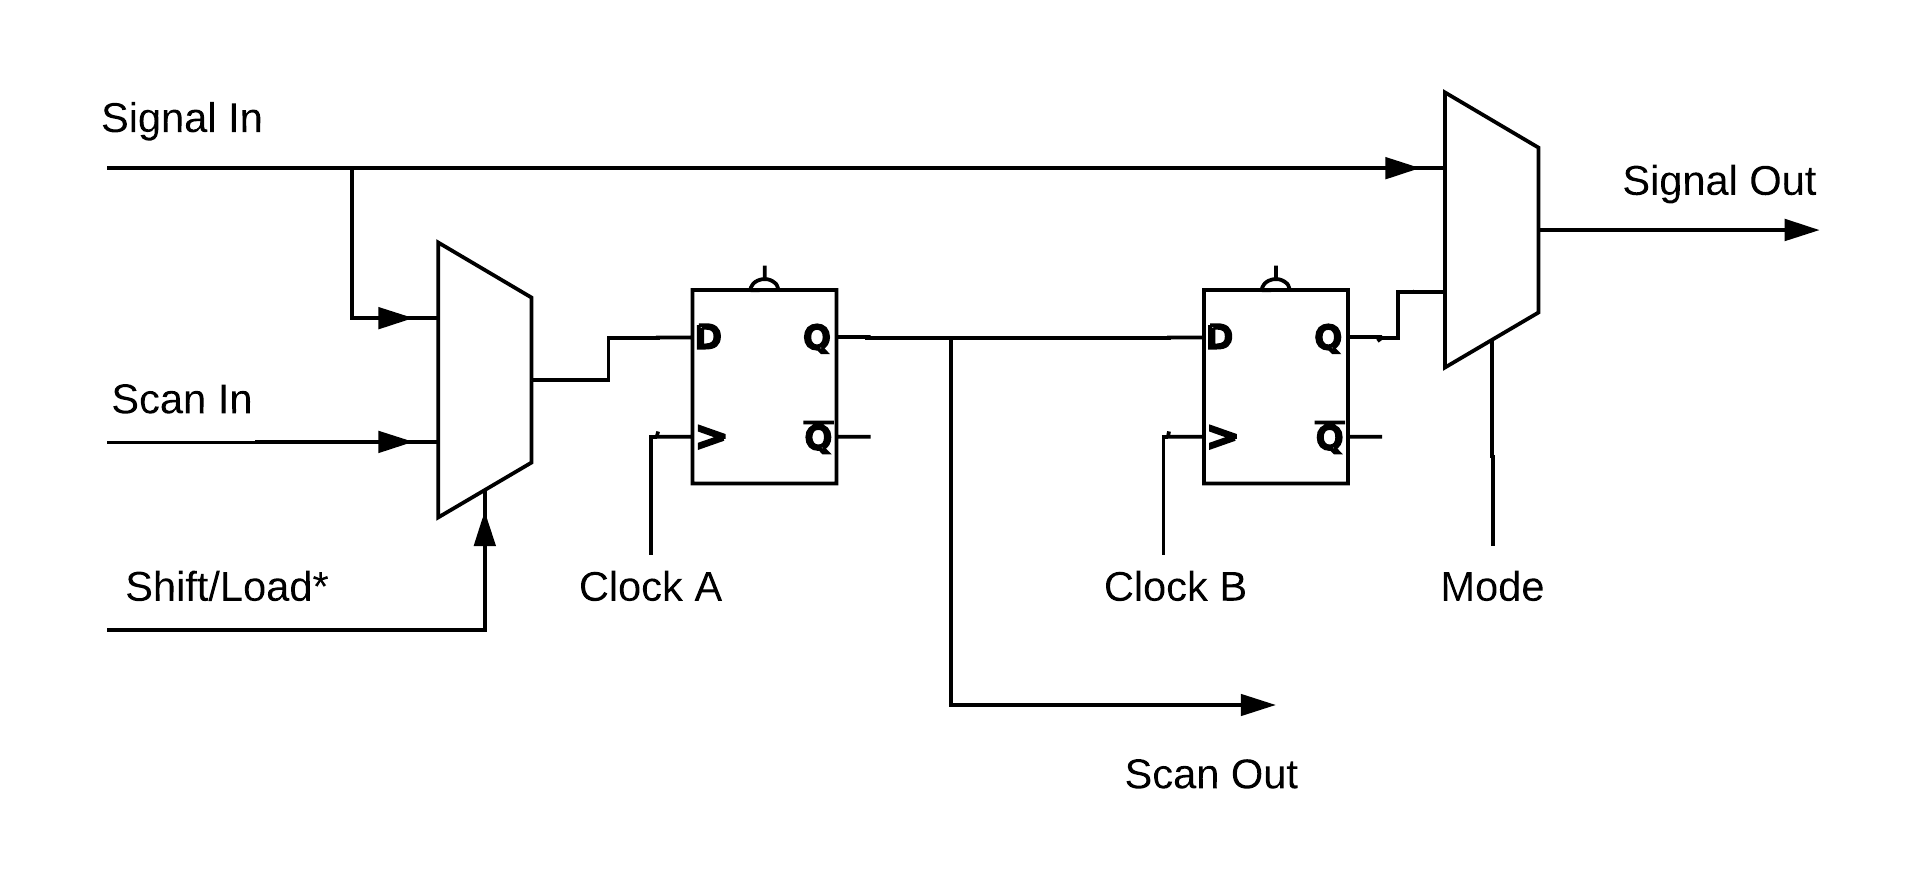
\includegraphics[width=0.8\linewidth]{fig/bscell}
            \caption{Célula de Verificação Periférica}
            \label{fig:bscell}
\end{figure}


O padrão IEEE 1149.1 se baseia em células de teste embutidas em todos os pinos de E/S do circuito integrado (figura \ref{fig:bscell}). As células são encadeadas em uma topologia em anel, em um esquema conhecido como \textit{daisy-chain}. O gerenciamento da cadeia de verificação é realizado pela porta de acesso ao teste (ou, em inglês, test acess port - TAP), permitindo que todos os pinos de E/S do integrado sejam acessíveis e testados pela porta JTAG. A figura \ref{fig:tap} mostra o esquemático conceitual da lógica interna da porta JTAG. A conexão em \textit{daisy-chain} entre os pinos de um dispositivo com suporte ao IEEE 1149.1 pode facilmente ser estendida para outros integrados compatíveis com o padrão, possibilitando o teste múltiplos integrados através de um único conector (figura \ref{fig:cadeiabs}). Como boa prática de DfM, recomenda-se a escolha de integrados que atendam ao padrão.

\begin{figure}
    \centering
        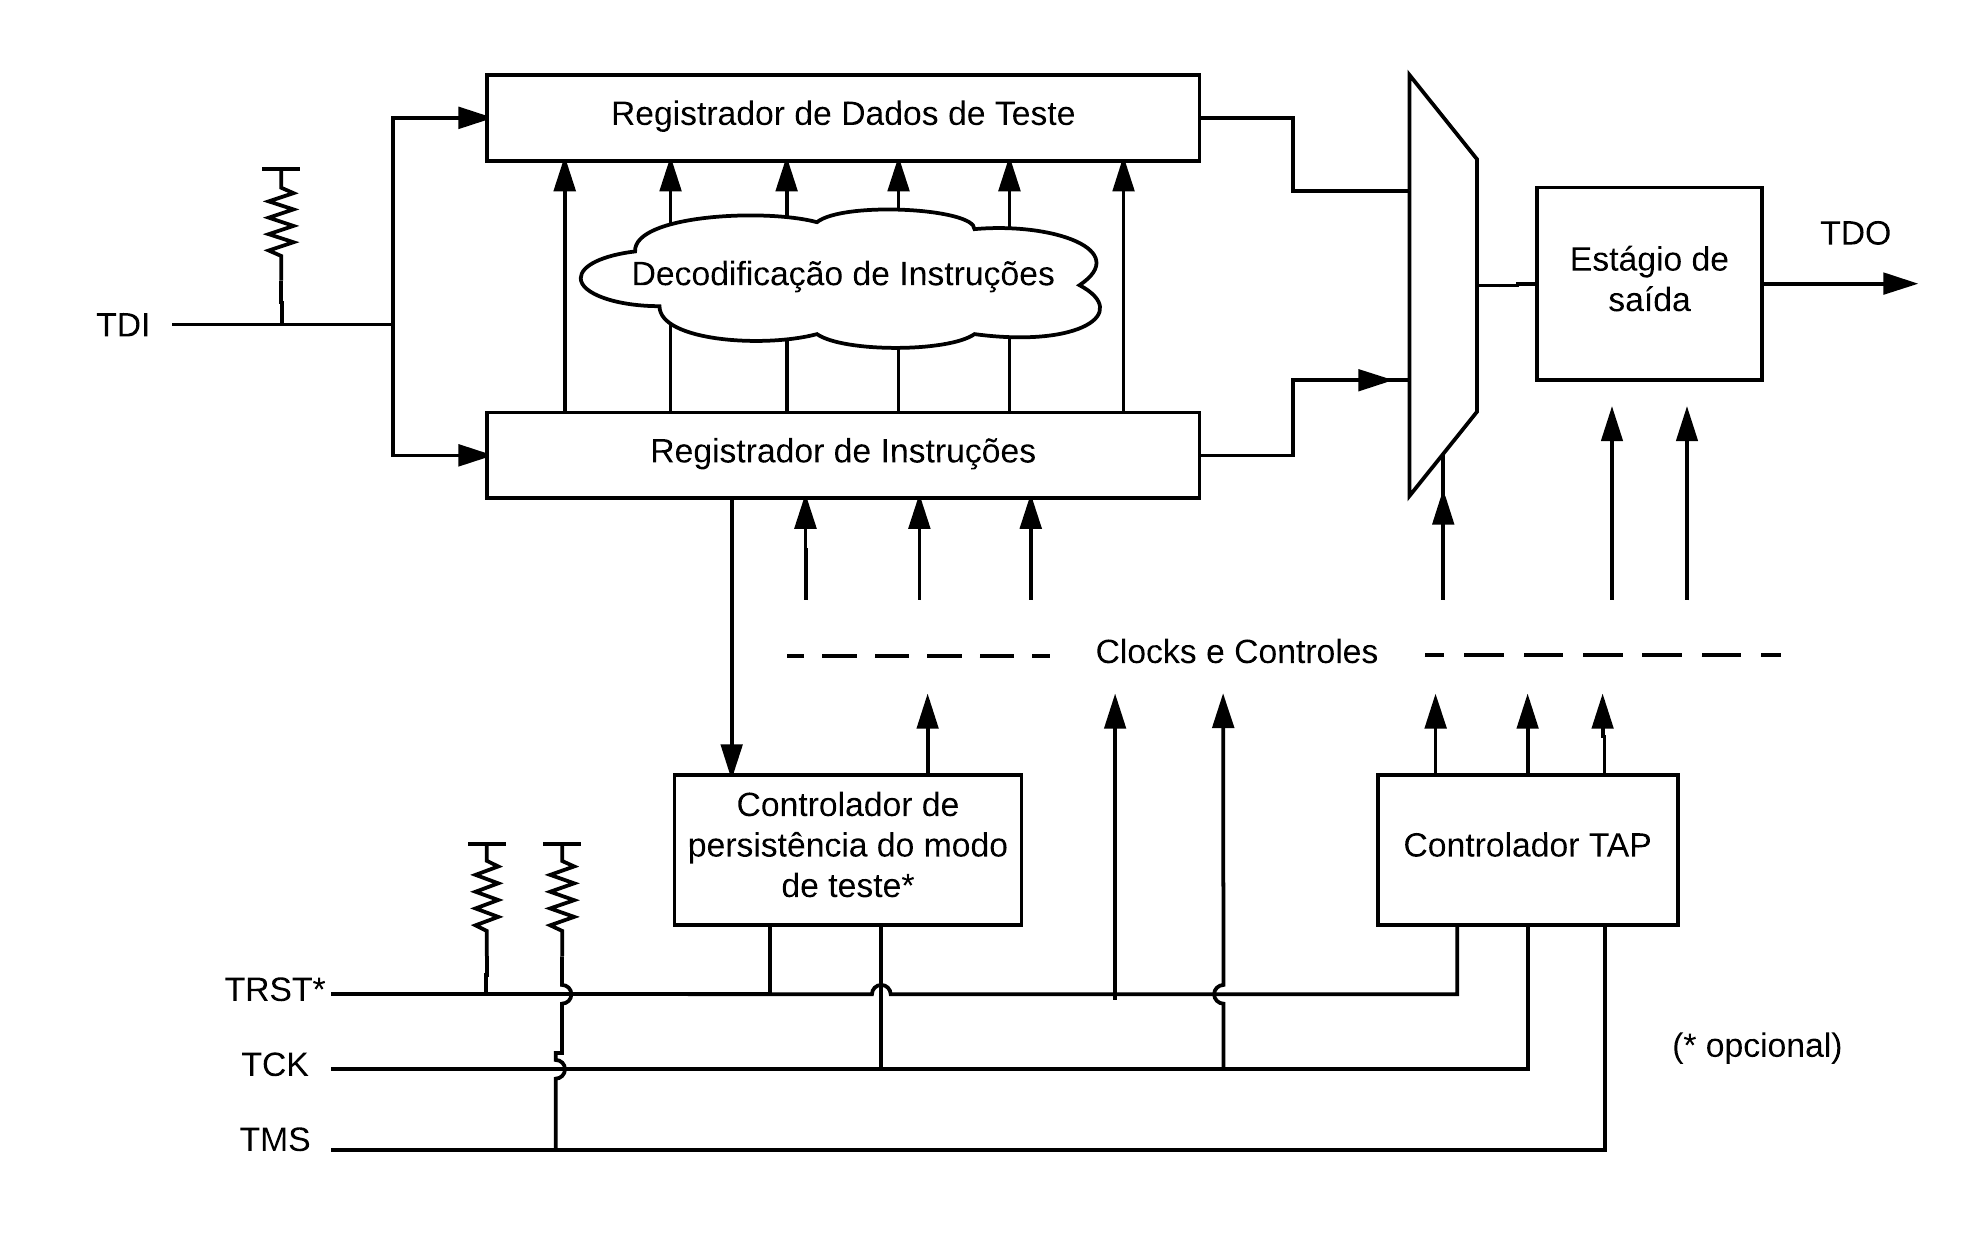
\includegraphics[width=1.0\linewidth]{fig/TAP}
            \caption{Esquemático conceitual da lógica de teste \textit{on-chip}}
            \label{fig:tap}
\end{figure}

Outro componente importante do JTAG, é a linguagem de descrição de varredura periférica (BSDL em inglês), que foi inserida numa revisão posterior do IEEE 1149.1 \citep{ieee11491de94}. A BSDL é um subconjunto do VHDL e é voltada para a descrição da infraestrutura de teste de um CI com o objetivo de tornar mais consistente a geração de testes e toda a cadeia de desenvolvimento envolvida nisso.

\begin{figure}
    \centering
        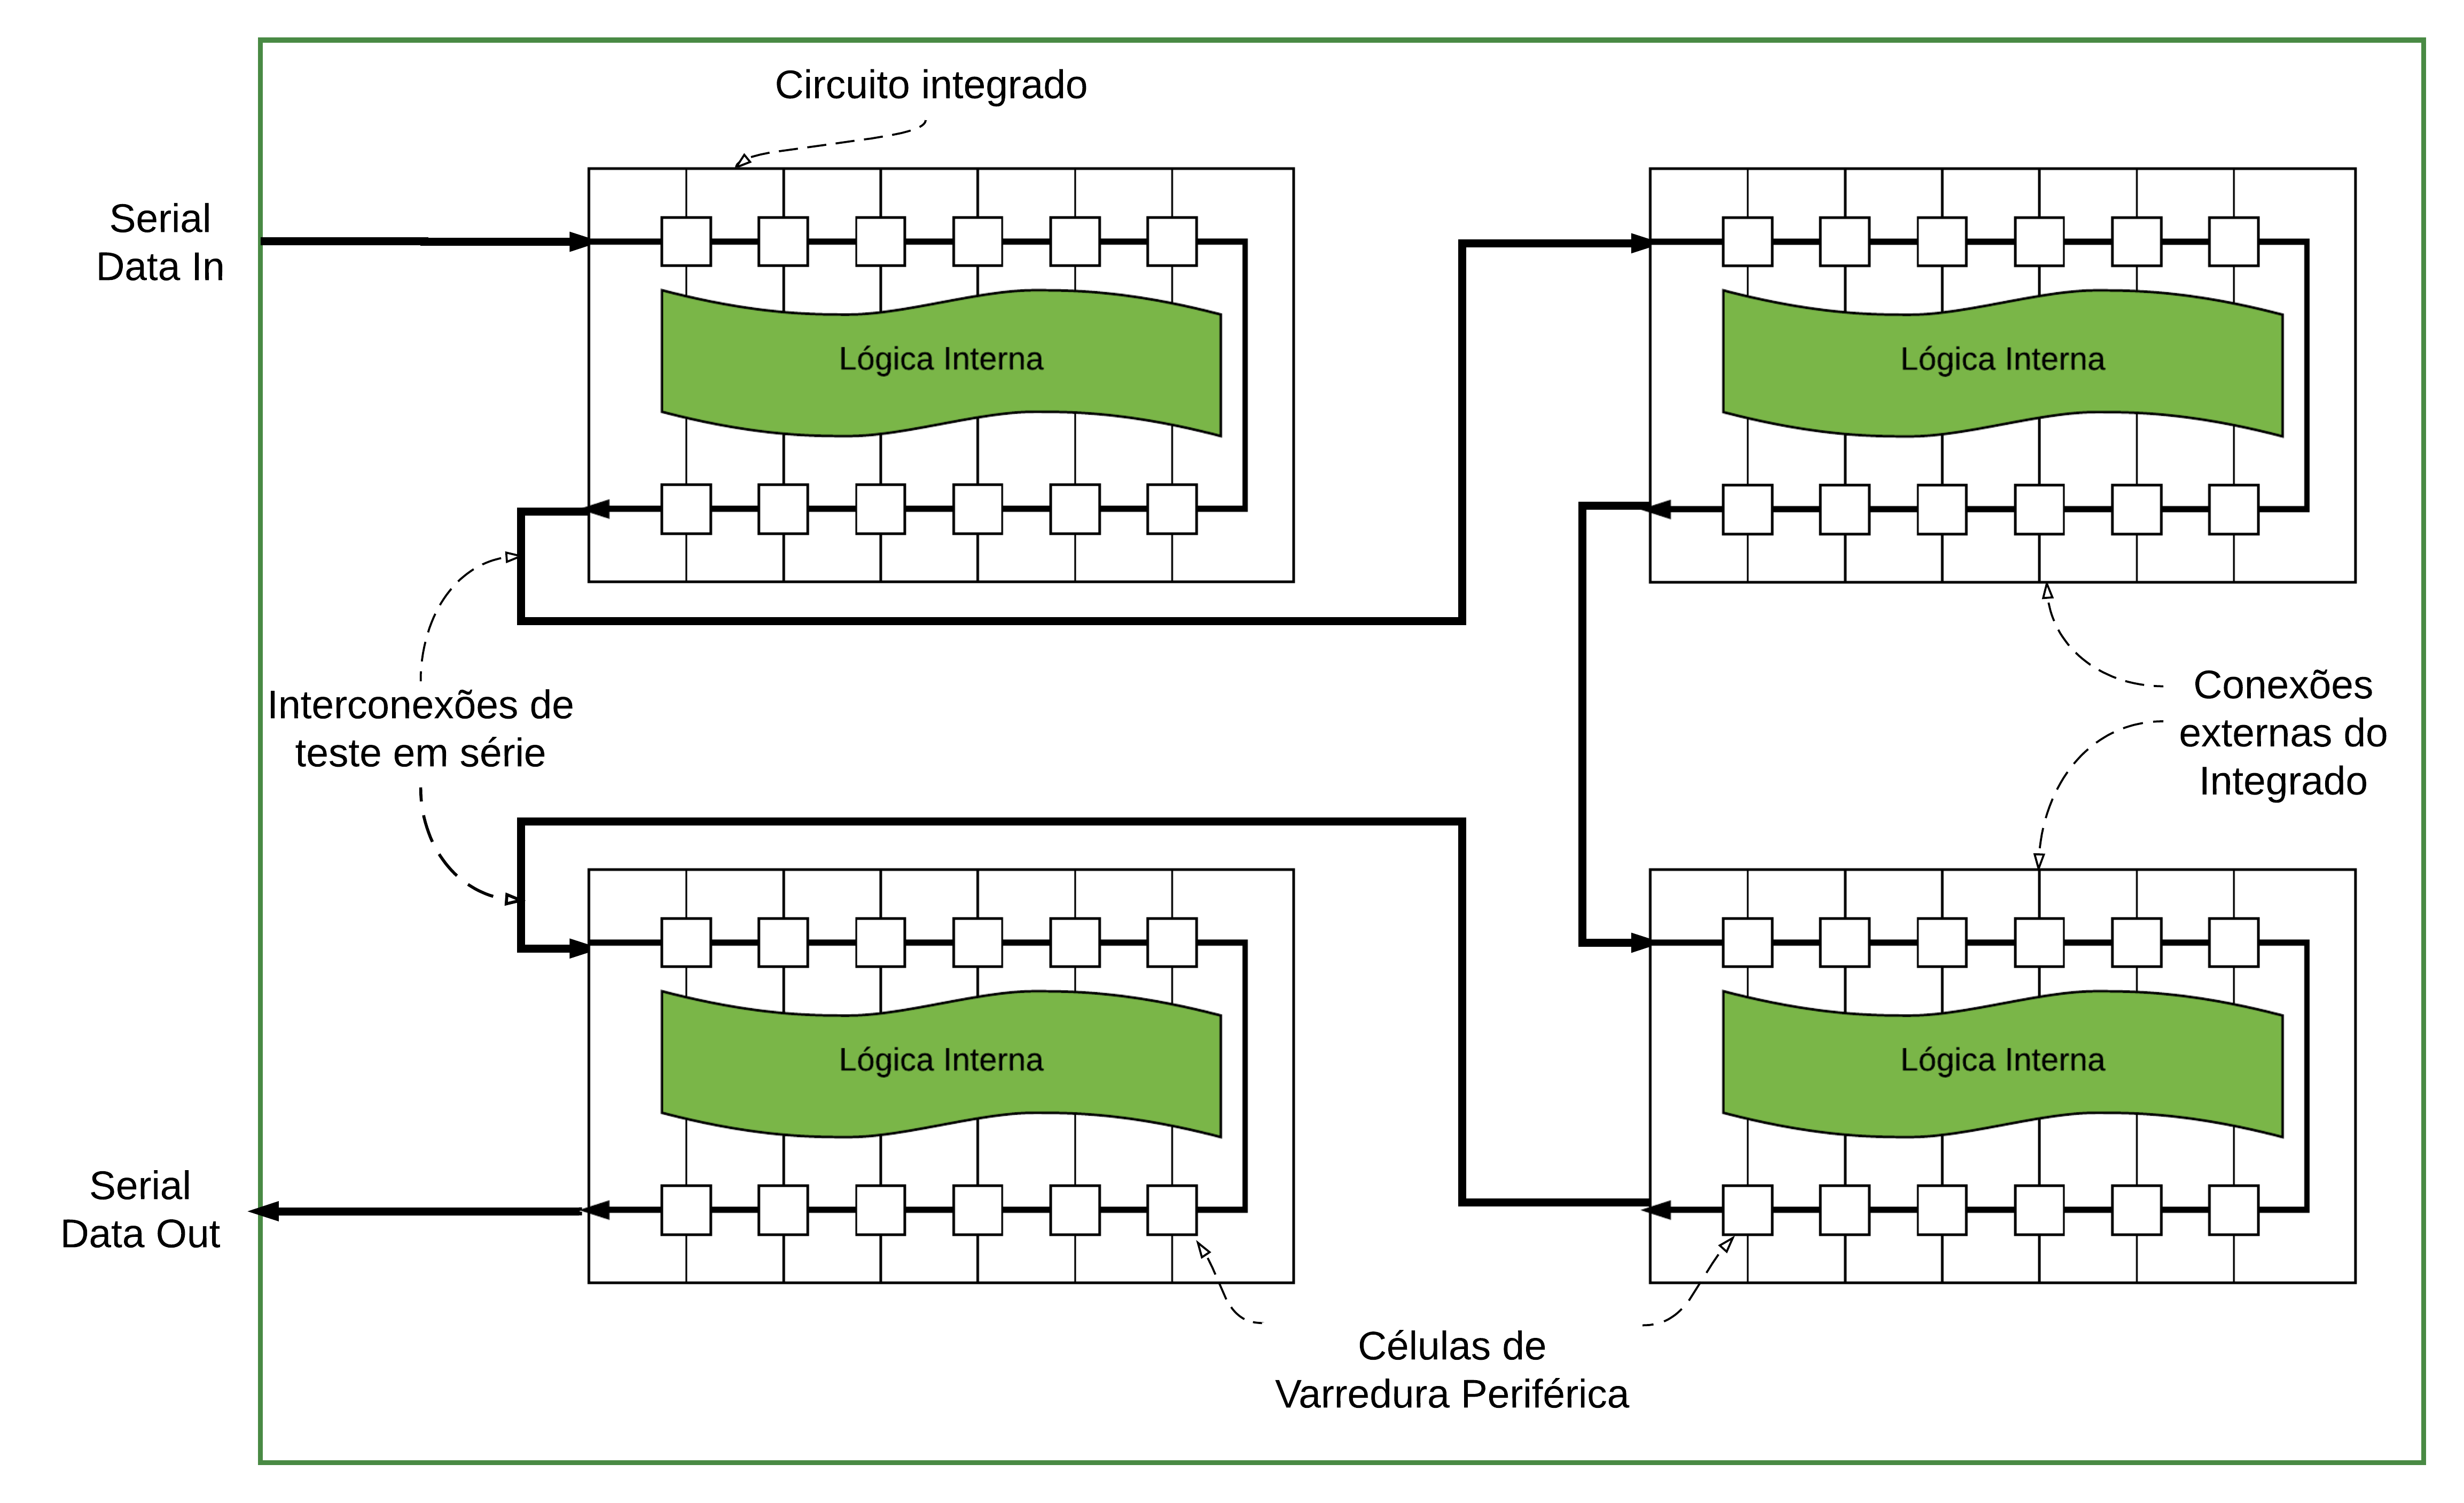
\includegraphics[width=1.0\linewidth]{fig/cadeiabs}
            \caption{PCI com as portas JTAG em \textit{daisy-chain}}
            \label{fig:cadeiabs}
\end{figure}


O padrão IEEE 1149.1 serviu de base para a criação de uma família de padrões de varredura periférica, e são exibidos na tabela \ref{tab:boundaryscanfamily} - adaptada de \citet{jutman2014high}.  

\begin{table}[h]
\centering
\tiny
\caption{Padrões IEEE baseados em varredura periférica}
\label{tab:boundaryscanfamily}
\begin{tabular}{p{50}p{50}p{50}p{50}}
\hline
\rowcolor[HTML]{C0C0C0} 
\multicolumn{1}{|p{50pt}|}{\cellcolor[HTML]{C0C0C0}\textbf{Foco principal de aplicação}} & \multicolumn{1}{p{50pt}|}{\cellcolor[HTML]{C0C0C0}\textbf{Propósito Principal}} & \multicolumn{1}{p{50pt}|}{\cellcolor[HTML]{C0C0C0}\textbf{Base da Tecnologia}}    & \multicolumn{1}{p{50pt}|}{\cellcolor[HTML]{C0C0C0}\textbf{Classes de falta a serem cobertas}}     \\
\rowcolor[HTML]{656565} 
\multicolumn{4}{|l|}{\cellcolor[HTML]{656565}{\color[HTML]{FFFFFF} \textbf{IEEE 1149.1 - Boundary Scan \citep{ieee11491old, ieee11491yr2013}}}}                                                                                        \\
\multicolumn{1}{|p{50pt}|}{Teste de Manufatura de PCI}                                        & \multicolumn{1}{p{50pt}|}{Melhorias de acesso aos testes}                               & \multicolumn{1}{p{50pt}|}{Registradores de sondagem on-chip}                            & \multicolumn{1}{p{50pt}|}{Faltas em pinos e integridade de circuto}                                 \\
\rowcolor[HTML]{656565} 
\multicolumn{4}{|l|}{\cellcolor[HTML]{656565}{\color[HTML]{FFFFFF} \textbf{IEEE 1149.4 - Barramento para testes de sinais mistos \citep{ieee11494}}}}\\

\multicolumn{1}{|p{50pt}|}{Medição de sinais analógicos} &
\multicolumn{1}{p{50pt}|}{Melhorias de acesso aos testes} & 
\multicolumn{1}{p{50pt}|}{Chaves \textit{on-chip}} &
\multicolumn{1}{p{50pt}|}{Valores paramétricos}\\

\rowcolor[HTML]{656565} 
\multicolumn{4}{|l|}{\cellcolor[HTML]{656565}{\color[HTML]{FFFFFF} \textbf{IEEE 1149.6 - Teste BST de Redes Digitais Avançadas \citep{ieee11496}}}}\\

\multicolumn{1}{|p{50pt}|}{Teste de redes LVDS de alta velocidade} &
\multicolumn{1}{p{50pt}|}{Teste de malhas acopladas em corrente alternada} & 
\multicolumn{1}{p{50pt}|}{Geradores de pulsos \textit{on-chip}} &
\multicolumn{1}{p{50pt}|}{integridade de malha}\\

%\rowcolor[HTML]{656565} 
\multicolumn{4}{|l|}{\cellcolor[HTML]{656565}{\color[HTML]{FFFFFF} \textbf{IEEE 1149.7 - Pinos reduzidos e TAP aprimorado \citep{ieee11497}}}}\\

\multicolumn{1}{|p{50pt}|}{Teste de placa e depuração de software} &
\multicolumn{1}{p{50pt}|}{Acesso à teste flexivel e em alta velocidade por dois pinos} & 
\multicolumn{1}{p{50pt}|}{SERDES, endereçamento} &
\multicolumn{1}{p{50pt}|}{Contempla todos acima}\\

%\rowcolor[HTML]{656565} 
\multicolumn{4}{|l|}{\cellcolor[HTML]{656565}{\color[HTML]{FFFFFF} \textbf{IEEE 1149.8.1 - Alternância de pinos e sensoriamento sem contato\citep{ieee114981}}}}\\

\multicolumn{1}{|p{50pt}|}{Teste de interconexão de PCIM} &
\multicolumn{1}{p{50pt}|}{Ligações para componentes passivos} & 
\multicolumn{1}{p{50pt}|}{chapas de sensoriamento capacitivo} &
\multicolumn{1}{p{50pt}|}{Circuitos abertos: AC e DC }\\

\multicolumn{4}{|l|}{\cellcolor[HTML]{656565}{\color[HTML]{FFFFFF} \textbf{IEEE P1149.10- TAP de alta velocidade \citep{ieeep1149102016} }}}\\

\multicolumn{1}{|p{50pt}|}{O mesmo que todos acima} &
\multicolumn{1}{p{50pt}|}{Permutação de dados de teste em alta velocidade} & 
\multicolumn{1}{p{50pt}|}{Reuso de pinos I/O de alta velocidade} &
\multicolumn{1}{p{50pt}|}{O mesmo que todos acima}\\

\multicolumn{4}{|l|}{\cellcolor[HTML]{656565}{\color[HTML]{FFFFFF} \textbf{IEEE 1500 - Teste de núcleo embarcado \citep{ieee1500}}}}\\

\multicolumn{1}{|p{50pt}|}{Teste à nível de SoC e IP} &
\multicolumn{1}{p{50pt}|}{Acesso ao teste de \textit{IP cores} em um SoC} & 
\multicolumn{1}{p{50pt}|}{invólucros de núcleos} &
\multicolumn{1}{p{50pt}|}{Faltas no domínio digital dentro de um CI}\\

\multicolumn{4}{|l|}{\cellcolor[HTML]{656565}{\color[HTML]{FFFFFF} \textbf{IEEE 1687 - Acesso por Instrumentação Embarcada \citep{ieee1687}}}}\\

\multicolumn{1}{|p{50pt}|}{Teste de CI, depuração, diagnóstico} &
\multicolumn{1}{p{50pt}|}{Padrão de acesso por instrumento} & 
\multicolumn{1}{p{50pt}|}{Cadeias de sonda reconfiguráveis} &
\multicolumn{1}{p{50pt}|}{Específicas do instrumento}\\

\multicolumn{4}{|l|}{\cellcolor[HTML]{656565}{\color[HTML]{FFFFFF} \textbf{IEEE P1838 - Acesso a teste para CIs 3D \citep{ieeep18382016}}}}\\

\multicolumn{1}{|p{50pt}|}{Teste de integração 3DSIC} &
\multicolumn{1}{p{50pt}|}{Acesso à teste através das vias TSV} & 
\multicolumn{1}{p{50pt}|}{O mesmo que os padrões 1500, 1149.1, 1687} &
\multicolumn{1}{p{50pt}|}{Integridade das vias TSV}\\
\hline


\end{tabular}
\end{table}

O padrão IEEE 1149.4 \citep{ieee11494} foi criado para testes paramétricos de componentes passivos, resistores pull-ups, componentes ativos como diodos transistores e de redes de impedância. Serve como uma extensão da varredura periférica para sinais analógicos. Este padrão ainda tem um número limitado de dispositivos compatíveis.

Já o padrão IEEE1149.6 \citep{ieee11496} estende a varredura periférica a portas de comunicação com acoplamento em corrente alternada, como por exemplo portas que atendem ao padrão de LVDS, operando em paralelo com os padrões 1149.1 e 1149.4. O que possibilita esta tecnologia são a inserção de geradores de pulso nos pinos de saída e receiver CA comuns e diferenciais nas entradas dos dispositivos que dão suporte a este padrão.

É possível citar outros exemplos significativos, como é o caso do IEEE1149.7 - cJTAG \citep{ieee11497}. Este padrão opera em pinos reduzidos e possibilita uma topologia em estrela ao invés do daisy-chain, permitindo um acesso mais rápido, além de oferecer uma infraestrutura adicional de suporte a tecnologias mais avançadas. O IEEE P1687 \citep{ieee1687} introduz o conceito de instrumentação embarcada para a aplicação de tarefas de teste, medição e diagnóstico, ao qual falaremos na próxima seção.

\subsection{Teste Controlado por FPGA ou Processador e Instrumentação Embarcada}
\label{FCT}

Conforme mencionado anteriormente, o JTAG não permite o uso de padrões de teste em velocidade nominal, deixando a classe de falhas de desempenho sob responsabilidade de testes funcionais. Atualmente, parte da indústria tem utilizado os componentes centrais de seus sistemas, como por exemplo os FPGAs e microcontroladores, como dispositivos de teste embarcado \citep{alcrouch2011, thomaswenzel2013}, cunhando os termos \textit{FPGA-Controlled Test - FCT} e \textit{Processor-Controlled Test - PCT}. 

 Além de cobrir os testes em domínio CA, como atrasos e \textit{crosstalk}, ainda possibilitam um acesso de baixo no nível no sistema, já que esses componentes normalmente são centrais. O custo marginal é ínfimo, já que o todo o \textit{hardware} de teste é reutilizado do produto e a memória de teste é apagada voltando o dispositivo para sua funcionalidade original. \citet{jutman2014high} afirmou que ainda são poucas as empresas fornecem ferramentas automatizadas para essa classe de testes.

O conceito de teste controlado por FPGA é possibilitado pelo uso de instrumentos embarcados, que definem-se como qualquer estrutura lógica dentro de um dispositivo cuja função é de teste, diagnóstico, \textit{Design for Testability (DfT), Design for Debug  (DfD), Design for Yield (DfY),} etc. Neste escopo enquadram-se diversas estruturas lógicas:    
\begin{itemize}
    \item Testadores de memória e BIST/BISD;
    \item Analisadores de taxa de erro (BERT) em canais de comunicação;
    \item Geradores de padrões de teste e \textit{buffers} de captura digital;
    \item Caracterizadores e Calibradores de E/S complexas;
    \item Testadores de barramentos de comunicação LAN SATA PCI CAN LIN I2C SPI e UART;
    \item Testadores sistêmicos e programação de memórias não voláteis;
    \item e Instrumentos definidos por usuário.
\end{itemize}

\citet{Stollon2011} mostra que estas estruturas de instrumentação embutida surgiram em parte pela necessidade de medições que causem menos interferências ou que comprometam a integridade do sinal de barramentos de alta velocidade internos ou externos ao CI. Dessa forma os fabricantes começaram a embutir núcleos de propriedade intelectual - \textit{IP cores} - de instrumentação interna permitindo testes não intrusivos e facilitando a validação e diagnóstico de placas.

Originalmente, cada um destes instrumentos são acessados e gerenciados por uma variedade de instrumentos externos, usando diversos mecanismos e protocolos. Isso dificulta a integração entre CIs e o reuso de tecnologia e equipamento. Logo, existia uma necessidade de padronização destes protocolos de forma a garantir uma metodologia eficiente e organizada para a preparação de testes e para o acesso e controle destes instrumentos embarcados. 

O IEEE 1687 \citep{ieee1687}- também conhecido como \textit{Internal JTAG} (IJAG), foi o padrão criado para definir e descrever as interfaces de acesso à instrumentação embarcada pela porta padrão IEEE1149.1, possibilitando a realização de testes avançados e não intrusivos em uma PCI inteira pela porta JTAG. Como ilustrado na figura \ref{fig:ieee1687}, o IJTAG não define os instrumentos ou suas funcionalidades por sí, mas sim os padrões de infraestrutura de acesso e como descrever os métodos e funcionalidades dos instrumentos. Isso se consolidou em duas linguagens de descrição dentro deste padrão: uma para as características destas funcionalidades, a PDL \textit{(procedural description language)}, e outra para os requerimentos de interface com estas funcionalidades - ICL \textit{(instrument connectivity language)}. Estas duas linguagens de descrição - PDL e ICL - facilitam o reuso e a descoberta de qualquer instrumento que seja compatível com o padrão IEEE 1687, independente do seu tipo, propósito ou origem. 

\begin{figure}
    \centering
        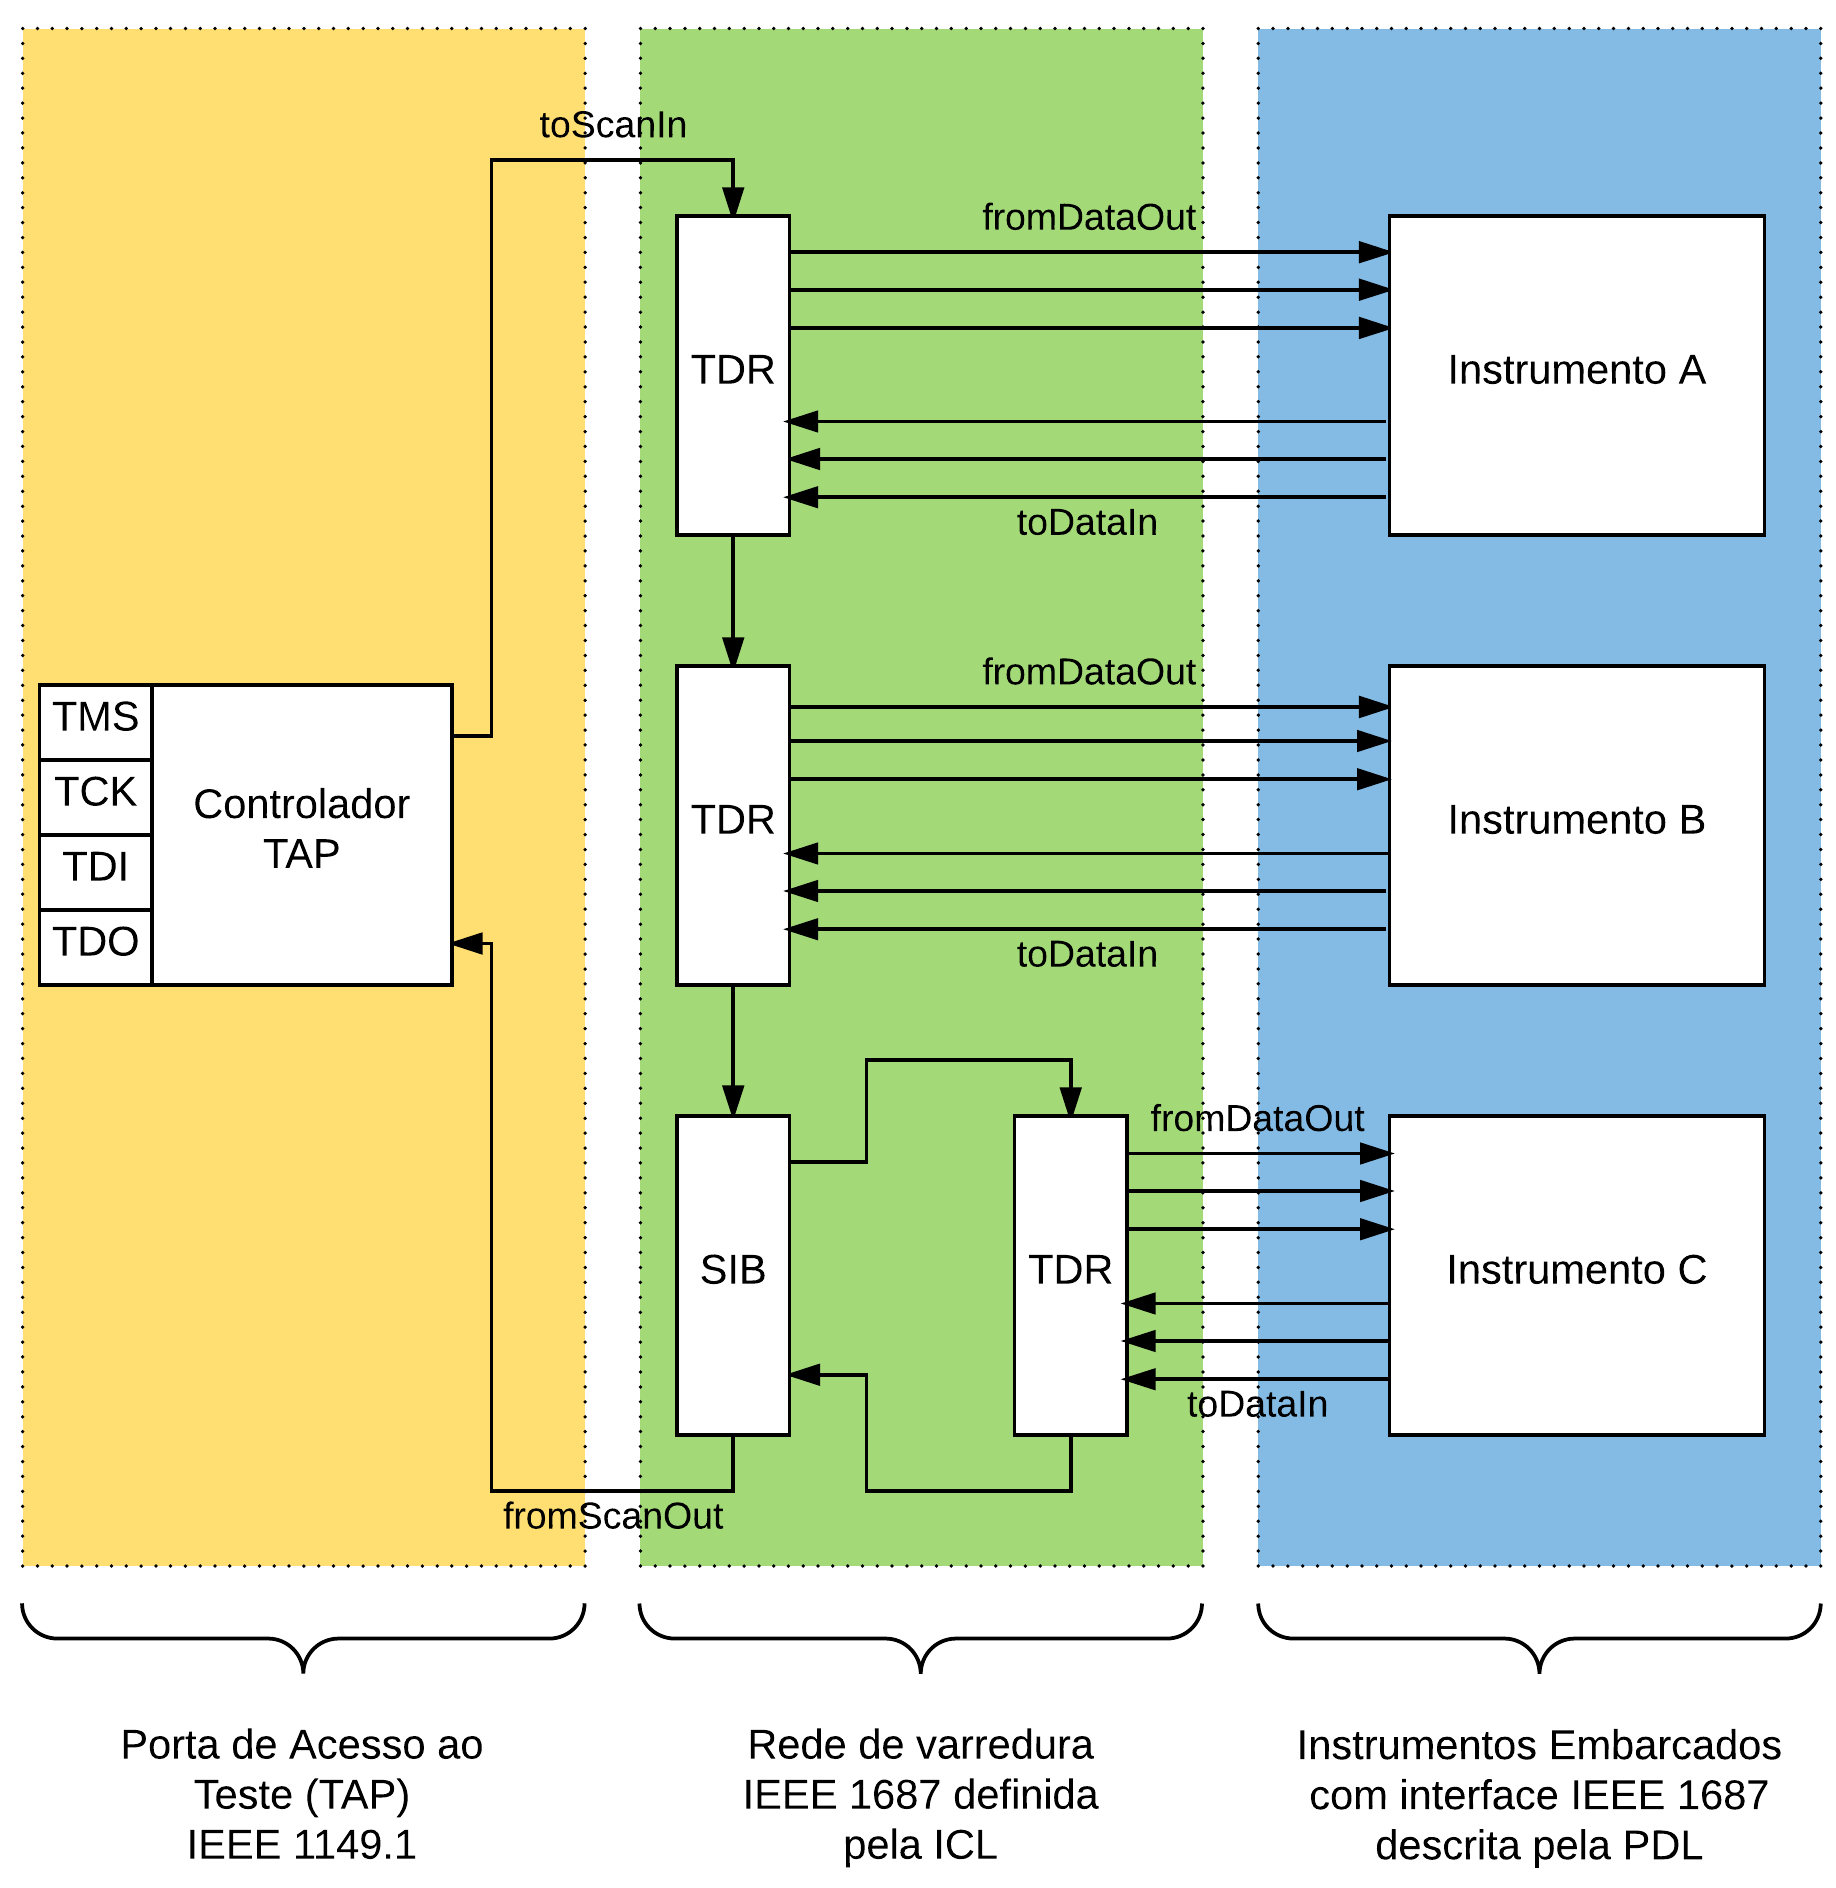
\includegraphics[width=1.0\linewidth]{fig/IEEE1687}
            \caption{Rede IEEE 1687 conceitual de multiplas cadeias de varredura}
            \label{fig:ieee1687}
\end{figure}

Dessa forma, o padrão IEEE 1687 funciona como uma estensão do IEEE 1149.1, de maneira que a porta JTAG de um CI ou uma placa possa ser usada para configurar, operar, e coletar dados de instrumentos embarcados.

Os FCT e PCT aliados ao IEEE 1687 oferecem uma cobertura de faltas em domínios em múltiplos domínios (estruturais, CC, CA, e faltas de desempenho), reduzindo ou até mesmo superando a necessidade de equipamentos de teste especializados \citep{thomaswenzel2013}. Em \citet{jutman2014high} observa-se que isso possibilita não só uma manufatura e teste de produção mais baratos e descomplicados, como também abre porta para o reuso dos testes em campo para o diagnóstico de falhas operacionais. O que não só reduz os custos logísticos de transporte de equipamentos especializados para depuração e diagnóstico, como possibilita que testes avançados sejam realizados sob condições reais de operação. 

\subsection{Teste Funcional}
% https://pad.riseup.net/p/RwPsE9imTtNzadskjasdoqidjefkadf
%definição
Define-se o teste funcional como um teste que não depende da estrutura interna de DfT de um sistema, mas sim das portas de entrada e saída \citep{jutman2014high}. Outra definição, formulada pelo mesmo autor, é a de um teste que se baseia somente nas informações funcionais do sistema, sem conhecimento da estrutura interna. Essas duas definições se interseccionam na maioria das vezes.

% contexto e papel do teste funcional em relação ao teste estrutarla
\citet{thibeault2006} mostra que o teste funcional em velocidade nominal tem sido usado para certificar CIs há mais de de 30 anos. Entretanto, devido às suas desvantagens, tem sido gradualmente substituído pelo teste estrutural como estratégia principal, a saber varreduras periféricas em velocidade nominal. A preocupação crescente com os crescentes custos de um teste funcional em velocidade nominal levou até a prever o seu desuso. 

Além disso, certos objetivos específicos de teste não podem ser cobertos por testes de varredura \citep{thibeault2006}.

Apesar de convenientes, os padrões mais avançados de varredura periférica e instrumentação embarcada ainda não chegaram a alcançar grande adesão pela indústria. 

\citet{tumim2001}

%objetivo  
% aplicações
A função do teste funcional é a de complementar objetivos específicos de teste, sendo normalmente empregado como etapa final de linha de produção \citep{jutman2014high}. Também mostram que existem diversas outras aplicações de testes funcionais. Citando: a inspeção de recebimento de componentes de terceiros (e.g.: uma fonte de alimentação feita por outro fabricante, ou circuito integrado de alto valor), e em casos de teste em campo do circuito eletrônico, quando se depende de equipamento externo especializado para a realização de testes ou o fabricante original do CI não disponibiliza o acesso à infraestrutura de teste interna.

Em \citep{thibeault2006} ve-se que que é importante considerar que, mesmo com suas vantagens, é crescentemente difícil justificar o uso de testes funcionais em velocidade nominal como abordagem principal. Sob esta perspectiva, parece que um teste funcional em velocidade nominal será mais e mais restrito à partes do DuT sem suporte à varredura periférica \citep{thibeault2006}. Todavia, a captura de defeitos relacionados á temporização não é o único aspecto positivo do teste funcional. Sua natureza não serial também pode ser explorada para propósitos de otimização de testes. Em [But100], foi proposto a criação de um pequeno conjunto de padrões de teste moderadamente rápidos, inseridos de inicio no programa de teste, de maneira a obter vantagem de sua inicial má capacidade de detecção de dispositivos enquanto mantem custos de desenvolvimento a um nível aceitável. Estas propostas foram baseadas no fato de qeu é mais difícil e caro criar e depurar padrões quando a frequência do  padrão funcional é perto da velocidade especificada do dispositivo.

Se estas classes de faltas em domínio CA e sistêmicas não forem corretamente tratadas, problemas sérios de \textit{falhas sem causa raiz} podem ocorrer, o que prejudica não somente a produção, como também põe a qualidade do produto em cheque. \citet{tumim2001} afirma que, mesmo com os últimos avanços nos testes de varredura periférica, o teste funcional ainda é insubstituível. A relação complementar entre essas duas categorias de teste é ilustrada pela figura \ref{fig:cobertura} adaptada de \citet{thomaswenzelenricozimmermann2016}. 

%vantagens
\citet{thibeault2006} enumera algumas das  principais vantagens e desvantagens do teste funcional. Dentre as vantagens destacam-se: a primeira é a possibilidade de execução de testes em velocidade nominal de operação, possibilitando a detecção de defeitos relacionados a temporização; A segunda é que os testes funcionais ainda são a maneira mais pratica de testar porções logicas para cobrir deficiências da varredura;

\citet{thibeault2006} também considera as desvantagens do teste funcional também:  O processo de teste funcional em velocidade nominal é muito mais demorado se comparado com a varredura periférica, especialmente se o objetivo é alcançar uma cobertura de teste superior aos 90\% [Tumi01]. A dificuldade e tempo requerido para gerá-los crescem exponencialmente em relação ao número de portas lógicas [Lin03].
 Por ultimo, Quando em velocidade nominal, os testes funcionais requerem alta velocidade de \textit{clock}, e muitas vezes serem operados em equipamentos mais caros [maxw00] 


%o que compõe
Como em qualquer problema de sistema em caixa preta, o teste funcional é composto pelos seguintes elementos: o roteiro de teste, os dados de excitação e os resultados e saída do teste.  A grande desvantagem da abordagem funcional é que mesmo que existam algoritmos para o teste funcional das estruturas lógicas mais comuns - como CPUs MMUs BPU, processadores multicores e GPUs - o esforço e tempo para geração deste teste podem ser significativos, como no caso de \citet{tumim2001}. Entretanto existem trabalhos mais recentes de automatização de testes funcionais como o de \citet{riefert2014effective} que desenvolveu um método automatizado para testes funcionais em processadores utilizando métodos formais.

O trabalho de \citet{thibeault2006} propõe uma investigação em otimização de roteiros e reuso de padrões de teste gerados diretamente por ferramentas de validação de projeto.

Em termos de teste funcional de interfaces com periféricos e interconexões, pode-se utilizar um ATE, para estímulos e observação, ou, caso o dispositivo esteja em campo e sem acesso a um ATE, pode-se usar uma conexão de loopback.

\section{Padrões de projeto em Labview}


Padrões de projeto são formas bem estabelecidas para resolver problemas comumente recorrentes. Não se trata de um código fonte ou framework, mas de uma descrição de como se resolver um problema que pode ser aplicado em diversas situações. Padrões de projeto ganharam popularidade na ciência da computação após a obra de Gamma et. al.\cite{gamma}, publicada em 1994. 

As vantagens de usá-los estão na facilidade dos desenvolvedores em reconhecê-los no código fonte, de dispensarem a necessidade de reinventar soluções para problemas recorrentes, como também na confiança de estar aplicando uma solução bem trabalhada para um tipo de problema.

No caso específico do Labview, os padrões de projeto podem ser um modelo como um framework, ou seja, uma base de código para o desenvolvimento da aplicação. São os padrões de projeto e frameworks mais conhecidos na linguagem: as máquinas de estado; os laços acionados por evento; o produtor-consumidor; o tratador de mensagem em fila; a máquina de estados em fila; e o Modelo de Atores;

As máquinas de estado são amplamente conhecidas e, nelas, o comportamento dinâmico do programa depende de estados cujas transições dependem de uma lógica de estados. É fundamental a criação de uma tabela de estados para uma máquina de estados efetiva.

<inserir figura representando este padrao>

Os laços acionados por eventos, diferentemente do paradigma procedural, a execução do programa é decidida em tempo de execução: o tratador de eventos espera que eventos ocorram para que executar seu tratador, poupando tempo de CPU. É uma boa alternativa ao uso de pooling e pode ser aplicada em qualquer sistema de acionamento de processos escravos.

% <inserir figura representando este padrao>

O produtor consumidor é normalmente aplicado quando se precisa executar tarefas assíncronas e comunicar entre elas sem perda de desempenho caso uma dependa da outra. Este padrão tem por característica a relação de mestre/escravo entre os laços, e a independência no fluxo de dados entre eles. Uma tarefa produzindo dados ou comandos e uma ou mais tarefas consumindo o que a produtora gera. A comunicação entre as tarefas é realizada por filas ou seja, os dados são enfileirados e desenfileirados em um buffer, em esquema conhecido como first-in-first-out - FIFO.

%<inserir figura representando este padrao>

O tratador de mensagens em fila (TMF) é uma extensão do produtor consumidor, possibilitando que processos escravos possam atuar também como produtores e comunicar entre si. Normalmente apresenta-se como na figura xxx, com um laço mestre acionado por eventos criando tarefas, um processo principal e subprocessos auxiliares. O TMF não só é um padrão de projeto, mas também a arquitetura base de muitas aplicações de média a grande complexidade. É aplicado em aplicações que exijam interfaces de usuário responsivas, aplicações multitarefa, e o desacoplamento de processos.

<inserir figura representando este padrao>

ACTOR FRAMEWORK

        \subsection{Framework de Atores}
            \label{actorframework}

Criado em 1973 por Hewitt, modelo de atores é um modelo conceitual para lidar com computação concorrente e sistemas distribuídos. Define algumas regras gerais de como os componentes de um sistema devem se comportar e interagir entre eles. 

Possui implementações em inúmeras linguagens, em paradigma orientado a objetos, como também no paradigma funcional. Em labview, sua implementação foi realizada por meio de um framework, ou seja uma estrutura básica de programa, no qual uma aplicação pode ser construída. É usado como solução de problemas de concorrência, principalmente em sistemas distribuídos.

A necessidade de um outro modelo de computação concorrente

Na programação imperativa, as threads são a solução tradicional para problemas de concorrência  na maior parte das linguagens de programação. Entretanto, programação concorrente baseada em threads, locks, e estados compartilhados são ditos difíceis de fazer e propenso a erro.

\subsubsection{Ator}

Um ator é a unidade primitiva de computação. É a coisa que recebe a mensagem e faz algum tipo de computação baseada nela.
A idéia é bem similar ao que existe em linguagens orientadas a objeto: Um objeto recebe uma mensagem (uma chamada de método) e faz algo dependendo de que tipo mensagem recebe (que método está chamando).
A grande diferença é que os atores são completamente isolados um do outro e eles nunca compartilham memória. É importante mencionar que um ator pode manter um estado privado que nunca poderá ser modificado diretamente por outro ator.

Um ator não é um ator, eles vêm em sistemas. No modelo de atores tudo é um ator e eles precisam de endereços, de forma que um ator pode enviar uma mensagem para outro.

Atores tem caixa de mensagens.
É importante entender que, mesmo que múltiplos atores possam ser executados ao mesmo tempo, um ator processará uma mensagem sequencialmente. Isso significa que se você enviar três mensagens ao mesmo tempo para um único ator, ele executará uma por vez. Para executar essas três mensagens concorrentemente, será necessário criar 3 atores e enviar uma mensagem para cada um.

Mensagens são enviadas de forma assíncrona para um ator, que precisa armazená-las em algum lugar enquanto está processando outra mensagem. A caixa de mensagem é o lugar onde estas mensagens são armazenadas.

O que atores fazem.

Quando um ator recebe uma mensagem, ele pode fazer 3 coisas:
Criar mais atores
Enviar mensagens para outros atores
Designar o que fazer com a próxima mensagem.

Os primeiros dois pontos são bem diretos, mas o último é interessante.
Foi dito anteriormente que um ator pode manter um estado privado. “Designar o que fazer com a próxima mensagem” basicamente significa definindo como este estado privado será para as próximas mensagens que o ator receber. De forma mais clara, é como os atores mutam seus estados.

Imagine que temos um ator que se comporta como uma calculadora e seu estado inicial é simplesmente o número 0. Quando o ator recebe a mensagem soma(1), ao invés de mutar seu estado original, ele designa que para as próximas mensagens que receber o estado vai ser 1.

Tolerância a Falhas

Outro aspecto do modelo de atores é a tolerância a faltas, no qual a política normalmente é deixar quebrar. A idéia por trás disso é que dispensa a necessidade de programar o sistema defensivamente, tentando antecipar todos os possíveis problemas que podem ocorrer e achar um modo de tratá-los. Simplesmente porque não há uma maneira de pensar em todos os pontos de falha.
O que normalmente se faz é simplesmente deixar quebrar e fazer com que este trecho crítico de execução seja supervisionado por alguém cuja única responsabilidade é saber o que fazer quando essa quebra ocorre, e o que faz tudo isso possível é o modelo de atores. Pelo fato dos atores serem completamente isolados uns dos outros, o estado de um ator não influenciará outros atores. Se um ator quebrar, seu supervisor, que também é um ator, será notificado e poderá fazer algo a respeito. 
Isso permite criar sistemas que se auto curem, de forma que se um ator do sistema quebrar, o sistema tem como detectar o problema e colocar o sistema em um estado consistente novamente (como resetar o ator em falha).

Distribuição
Um outro aspecto interessante do modelo de atores é que não importa se o ator que estou enviando uma mensagem está sendo executado localmente ou em outro nó da rede. Se um ator é uma parte de código com uma caixa de mensagens, um estado interno e só responde a mensagens, não importa aonde ele está localizado desde que a mensagem chegue aonde ele está. Isso permite a criação de sistemas com vários computadores e ajuda a recuperar o sistema caso um deles falhe.



Em resposta a uma mensagem que recebe, um ator pode: tomar decisões locais (dentro de seu domínio de atuação), criar mais atores, enviar mais mensagens, e determinar como responder às próximas mensagens (ver figura \ref{fig:actormodel}). Atores podem ter e mudar seus estados privados, mas só podem afetar um a outro por mensagens, dispensando o uso de \textit{locks} (mutex, semáforos, etc). 
            
             \begin{figure}
                \centering
                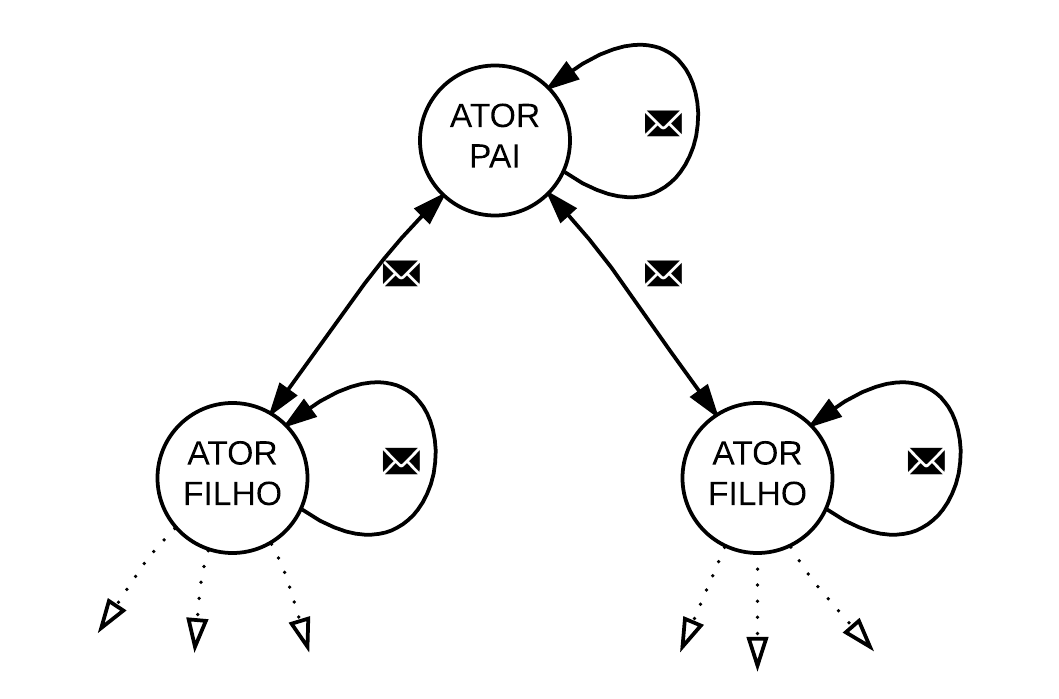
\includegraphics[width=0.9\linewidth]{fig/actormodel}
                \caption{Um exemplo ilustrativo de sistema com 3 atores e  as possibilidades de mensagens entre eles. Atores podem criar outros atores se necessário.}
                \label{fig:actormodel}
            \end{figure}
            
            
            %O que é, para o que serve e como funciona;        
            \subsubsection{Como funciona}
                Conforme falado, atores trabalham sempre em resposta às mensagens que recebem. Tais mensagens são armazenadas numa fila de dados para serem processadas uma de cada vez, num esquema FIFO ( \textit{First In, First Out} ou primeiro a entrar, primeiro a sair). Tal esquema está representado na figura \ref{fig:actor}.
            
                \begin{figure}
                    \centering
                    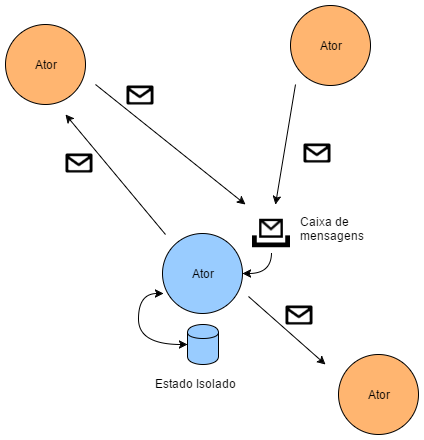
\includegraphics[width=0.9\linewidth]{fig/actor}
                    \caption{Funcionamento interno de um ator}
                    \label{fig:actor}
                \end{figure}
                
                Um ator pode enviar mensagens para o ator que o criou, atores que ele criou, e também para sí mesmo (ver figura \ref{fig:actormsg}).
                
                \begin{figure}
                    \centering
                    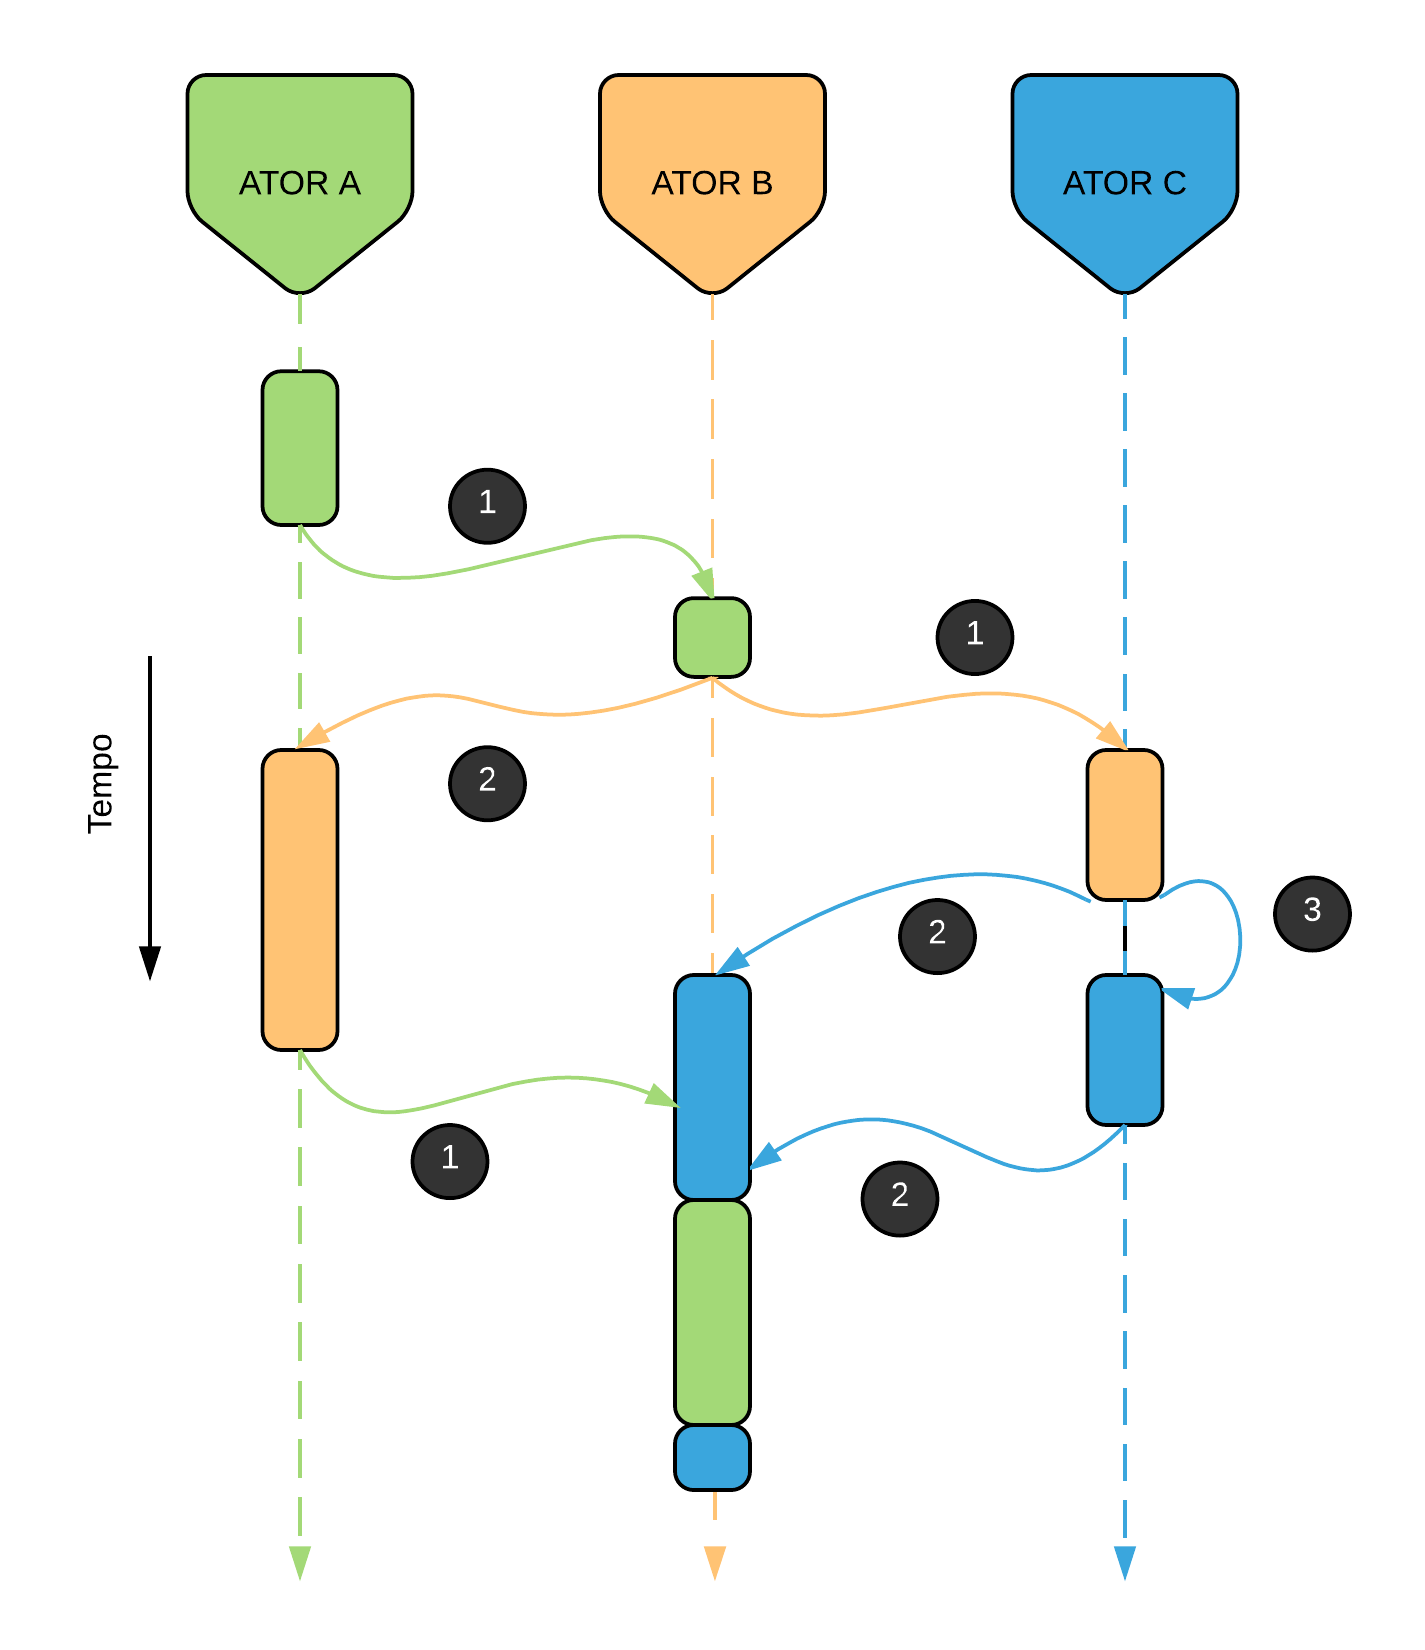
\includegraphics[width=0.9\linewidth]{fig/actormsg}
                    \caption{Mensagens no modelo do ator: (1) atores podem mandar mensagens para seus filhos; (2) atores podem mandar mensagem para os seus pais; (3) atores podem mandar mensagem para sí mesmos}
                    \label{fig:actormsg}
                \end{figure}
        
                Podemos perceber que os atores não compartilham estados entre eles, o que os tornam desacoplados uns dos outros. Ou seja cada ator é independente dos outros atores do sistema.
                
                %Comunicação Assíncrona.



REALITY CHECK - o que de técnica escolheu e da de usar

Em metodologia:
-> importante mencionar que também como forma de aprendizado em OOP e também o uso de framework complexos 
-> mencionar que dentro dos atores, foram usados diversos outros design patterns e estruturas


            Este framework foi escolhido por já ser uma estrutura bastante consolidada dentro do LabView, com uma comunidade de usuários extensa para dar suporte e por permitir escalar o processo de testes, transformando programas que executam roteiro de testes de forma sequencial em entidades cujos subdomínios podem ser executado em paralelo, mas com uma estrutura segura que previna \textit{deadlocks} de execução.
            
            Além disso, a modularidade dessa abordagem permite que, em caso de expansão do hardware de teste com o uso de jigas que suportem múltiplos DUT, a melhoria em software torna-se relativamente fácil, já que é possível instanciar mais atores com facilidade. Pode-se também instanciar atores em outros computadores e o sistema descentralizado funcionar como um só.
            Em resumo, é um framework consolidado, escalável, com um bom suporte e uma comunidade grande e diversa.



MENCIONAR QUE A PLACA N TEM JTAG E O CHIP È PROPRIETÁRIO E PRECISAMOS CONFIAR NO FABRICANTE
PROBLEMA DE BUGS QUE BOTARAM NO RABO DO SETOR DE QUALIDADE





O que eu quero falar na revisão?
Esta revisão bibliográfica pretende atingir dois objetivos: a revisão do estado da arte em placas eletrônicas, e também dos fundamentos do uso de programação concorrente, foco deste trabalho

Estrutura

Introdução (contextualização)
Revisão bibliografica ok
	Historica opcional
	Estado da arte ok
Definição/especificação do problema tratado
Metodologia
Materiais utilizados
Aplicação da metodologia à solução do problema
Resultados
Discussão dos resultados
Conclusão
Bibliografia
Anexos

O que eu quero falar na revisão?
Esta revisão bibliográfica pretende atingir dois objetivos: a revisão do estado da arte em teste de  placas eletrônicas, e também dos fundamentos do uso de programação concorrente, foco deste trabalho


Definir teste e diagnóstico.
Teste é o procedimento de checagem realizado para garantir a qualidade, desempenho, e confiabilidade de algo antes de ser colocado em uso
Diagnóstico é a identificação de uma causa raiz de um problema pela examinação de seus sintomas.
Metricas



